\chapter{Enhanced ECal reconstruction}
\label{chap:EnhancedECalReconstruction}
The current implementation of the ECal reconstruction software was designed to reconstruct particles which originate from the ND280 Tracker and enter the ECal.  As section~\ref{sec:ECalEventReconstruction} shows, this was realised by only considering reconstructed ECal clusters under the single track-like or shower-like hypothesis.  It should be evident that a neutrino interaction occurring within the ECal does not well fit this topology.  While it is true that there is some power in the current reconstruction to distinguish a neutrino interaction from an entering track or shower, there is little feature information available.  How many final state particles propagated from the interaction?  How much visible energy was deposited by each of the particles?  Where in the ECal did the interaction occur?  These basic questions can not be trivially answered when using the current reconstruction.  To maximise the ability of distinguishing ECal neutrino interactions from entering backgrounds, the reconstruction must be revisited.

\section{The Hough transform}
\label{sec:HoughTransform}
The Hough transform is a popular method of machine pattern recognition used by, but is not limited to, high energy physics experiments.  Originally designed for machine track recognition in bubble chamber pictures~\cite{Hough:1959qva}, the version most widely used throughout the world was developed in 1972~\cite{Duda:1972:UHT:361237.361242}.  The Hough transform is used to isolate specific features or shapes from a digital image.  The simplest implementation, which is of most interest in event reconstruction, allows the extraction of straight 2D lines from a complex pattern.  This is achieved by exploitation of a simple, but remarkable, feature of 2D geometry.

\subsection{Line-point duality}
\label{subsec:LinePointDuality}
Consider a straight line formed in a 2D Cartesian space as shown in Fig.~\ref{fig:2DCartesianLine}.  The line is usually described by
\begin{equation}
  y = mx + c
  \label{eq:2DLineCartesean}
\end{equation}
where $y$ and $x$ are used as coordinates, $m$ is the gradient of the line and $c$ is the intercept location of the line with the $y$ axis.  While it is not necessary to analyse this simple shape in great detail, it is important to note that $m$ and $c$ are the only parameters necessary to completely describe the line.  
\newline
\newline
Now consider a new 2D space where the axes are defined by $m$ and $c$, rather than $x$ and $y$ (hereafter referred to as the parameter space).  As this parameter space is described by the parameters of a general 2D Cartesian line, there is an underlying symmetry between the two spaces.  The parameters of the 2D line shown in Fig.~\ref{fig:2DCartesianLine} can be used to form a pair of coordinates ($m$, $c$) in the parameter space as shown in Fig.~\ref{fig:2DParameterPoint}.  It is important here to state clearly the general result; a straight line in Cartesian space is represented by a single point in parameter space. 
\begin{figure}%
  \centering
  \subfloat[Line in 2D Cartesian space.  The line is defined by its intercept with the $y$-axis, $c$, and its gradient, $\Delta y/\Delta x = m$ (not shown).]{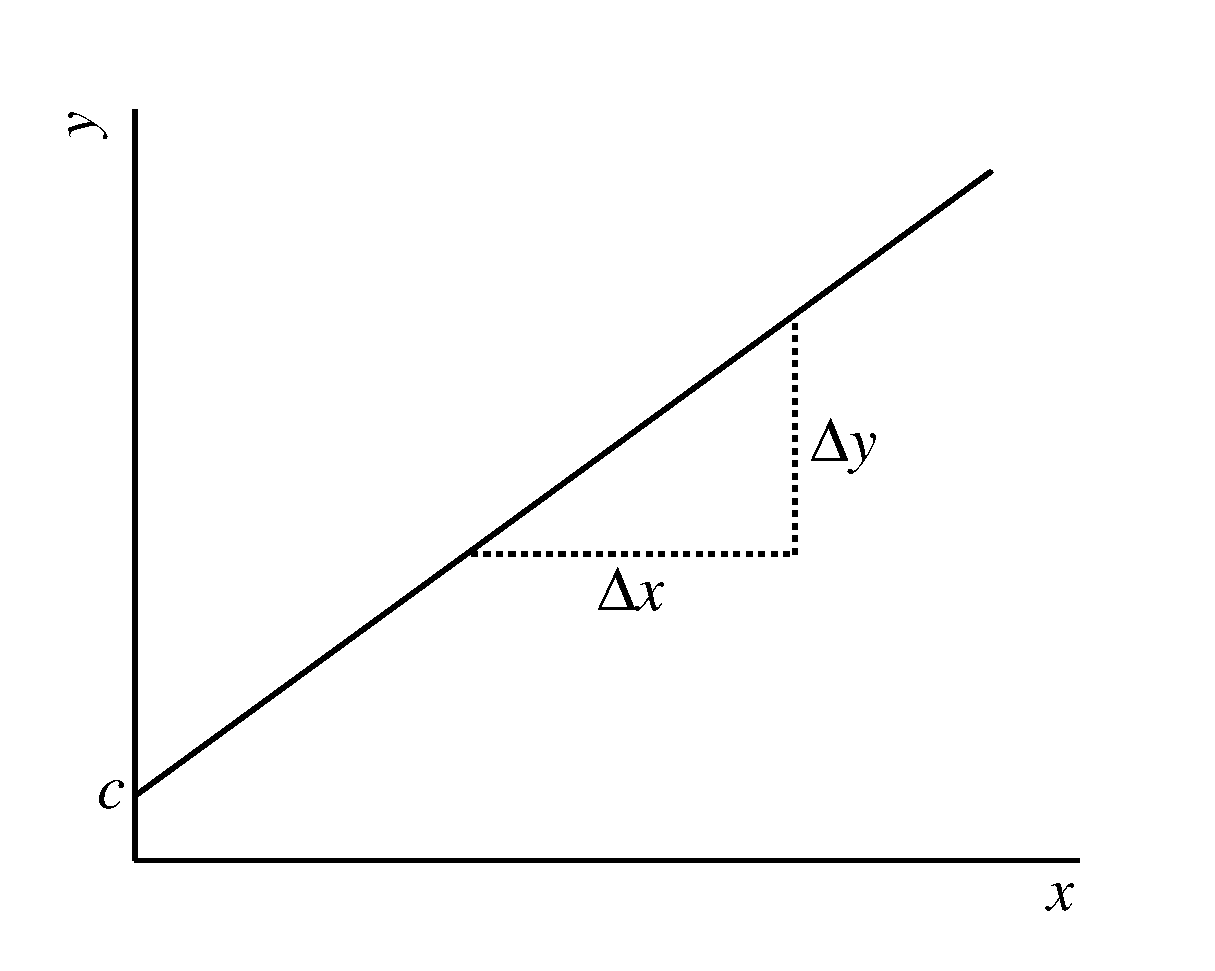
\includegraphics[width=7cm]{images/hough_transform/cartesian_line} \label{fig:2DCartesianLine}}
  \hspace{1em}
  \subfloat[Point representation of the line defined in Fig.~\ref{fig:2DCartesianLine} in 2D parameter space.  Because the line is solely defined by its intercept, $c$, and its gradient, $m$, the line is defined as a point in this parameter space.]{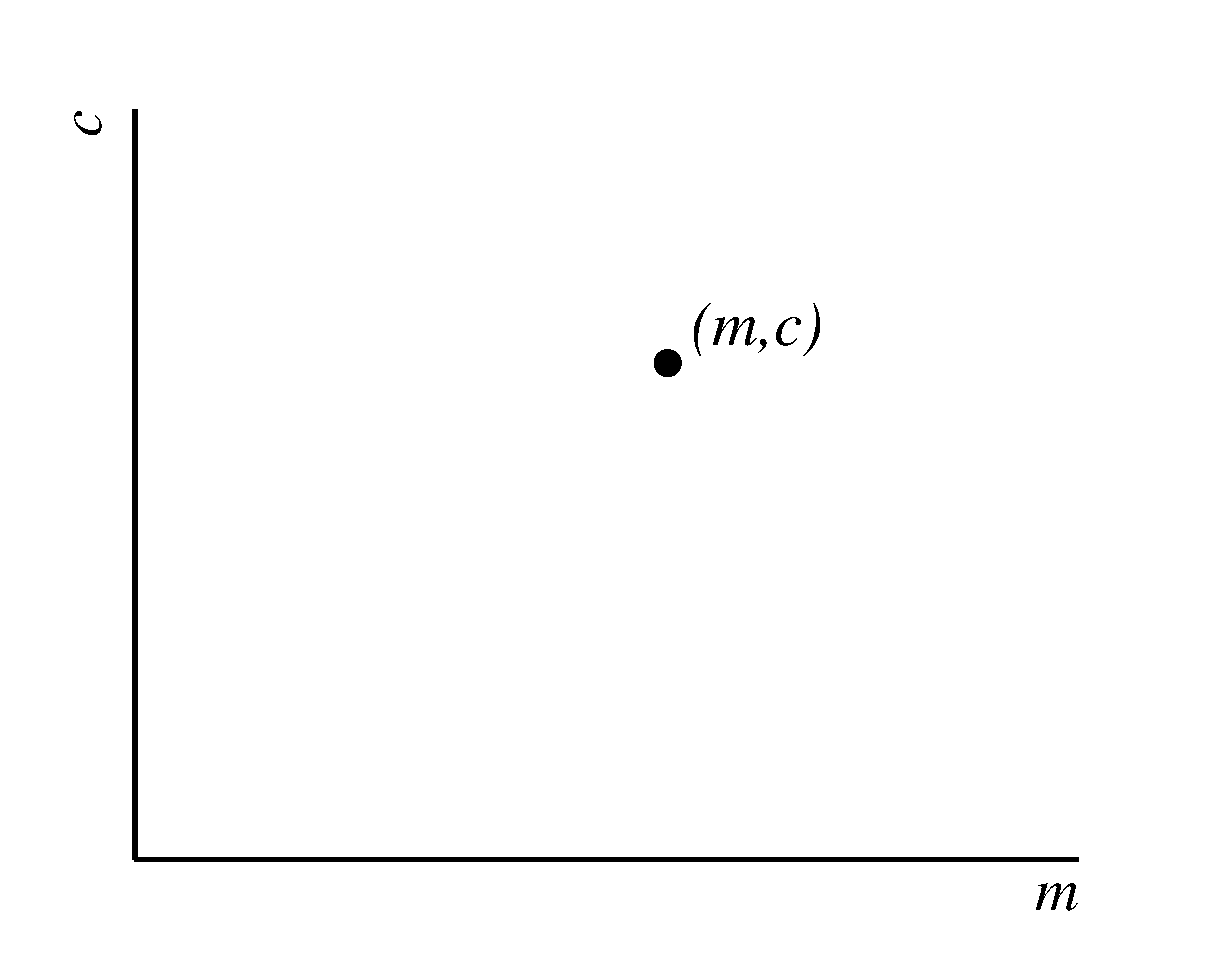
\includegraphics[width=7cm]{images/hough_transform/parameter_point} \label{fig:2DParameterPoint}}
  \caption{Representations of a 2D line in Cartesian space.}
  \label{fig:2DCartesianLineAndParameterPoint}
\end{figure}
\newline
\newline
Now consider the 2D Cartesian space again.  Unlike before, we will define a single point rather than a straight line. Such a point is traditionally described by a pair of coordinates ($x$, $y$).  However, an alternative description of the point is an infinite number of lines all of which pass through ($x$, $y$).  This is highlighted by Fig.~\ref{fig:2DCartesianPoint} where three lines of the infinite set are shown along with the point they represent.  As the infinite line set are used to describe a single point, all lines in the set must follow a pattern.  This relationship is revealed by simple algebraic manipulation of equation~\ref{eq:2DLineCartesean} to give
\begin{equation}
  c = -xm + y.
  \label{eq:2DLineParameter}
\end{equation}
Despite the manipulation, equation~\ref{eq:2DLineParameter} still resembles the equation of a 2D line\Yoshi{; however,}{ADDRESSED - was ``, however''; see \url{http://www.nationalpunctuationday.com/semicolon.html}} the parameters are $x$ and $y$ and the coordinates are $m$ and $c$.  Specifically, equation~\ref{eq:2DLineParameter} is represented by a line in the parameter space defined above.  The gradient of this line is 
\begin{equation}
  x = \frac{\Delta c}{\Delta m}
  \label{eq:2DLineGradientParameterSpace}
\end{equation}
and the intercept of the line with the $c$ axis is $y$ as shown in Fig.~\ref{fig:2DParameterLine}.  As before, it is important to clearly state what has been shown; a point in Cartesian space is represented by a line in parameter space.
\begin{figure}%
  \centering
  \subfloat[Point in 2D Cartesian space.  The point can be defined as an infinite set of lines, all of which cross at said point (three example lines are shown).]{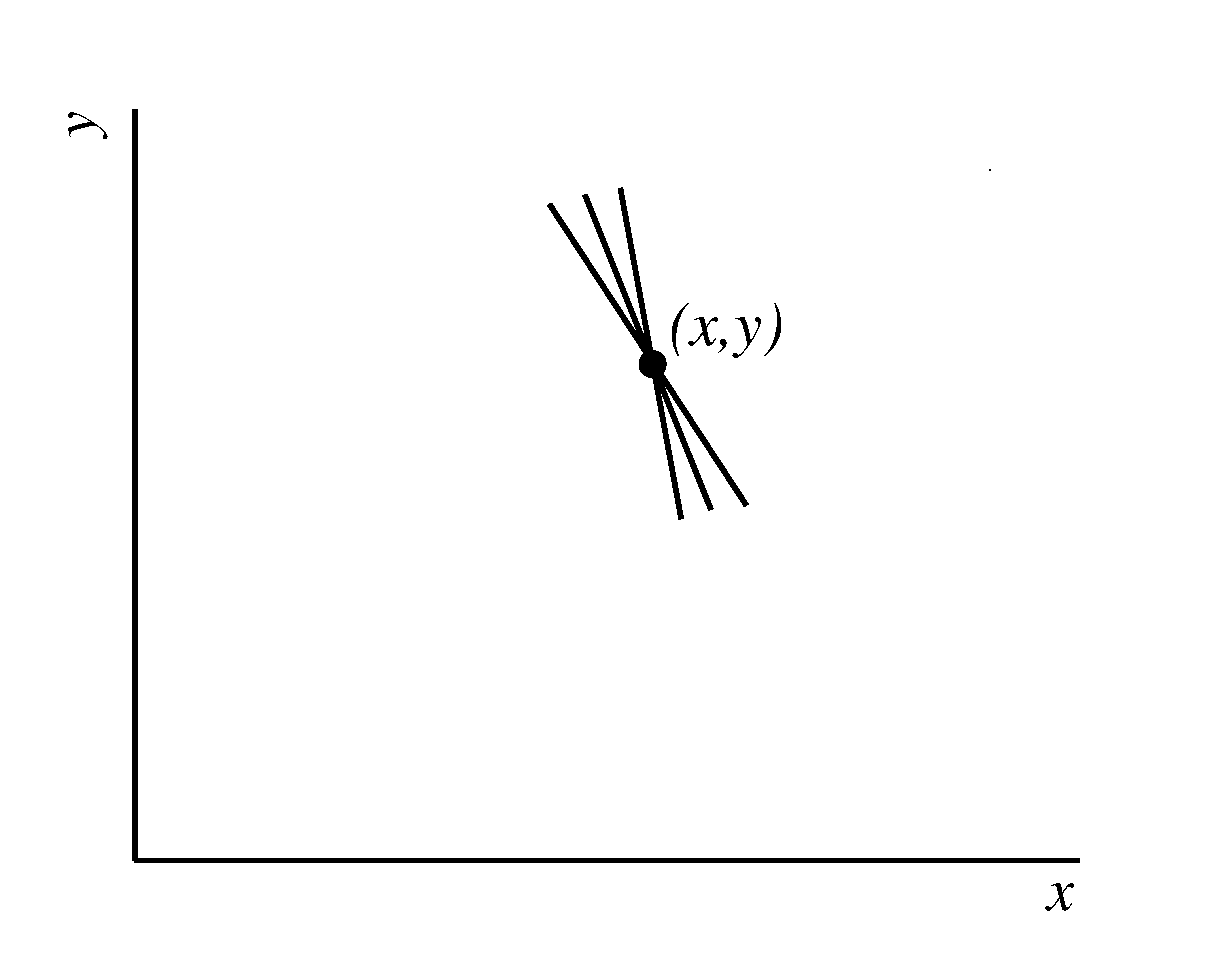
\includegraphics[width=7cm]{images/hough_transform/cartesian_point} \label{fig:2DCartesianPoint}}
  \hspace{1em}
  \subfloat[Line representation of the point defined in Fig.~\ref{fig:2DCartesianPoint} in 2D parameter space.  The infinite set of lines which represent the point in Fig.~\ref{fig:2DCartesianPoint} follow a relation, $c=-xm+y$, which itself is a line in the parameter space.]{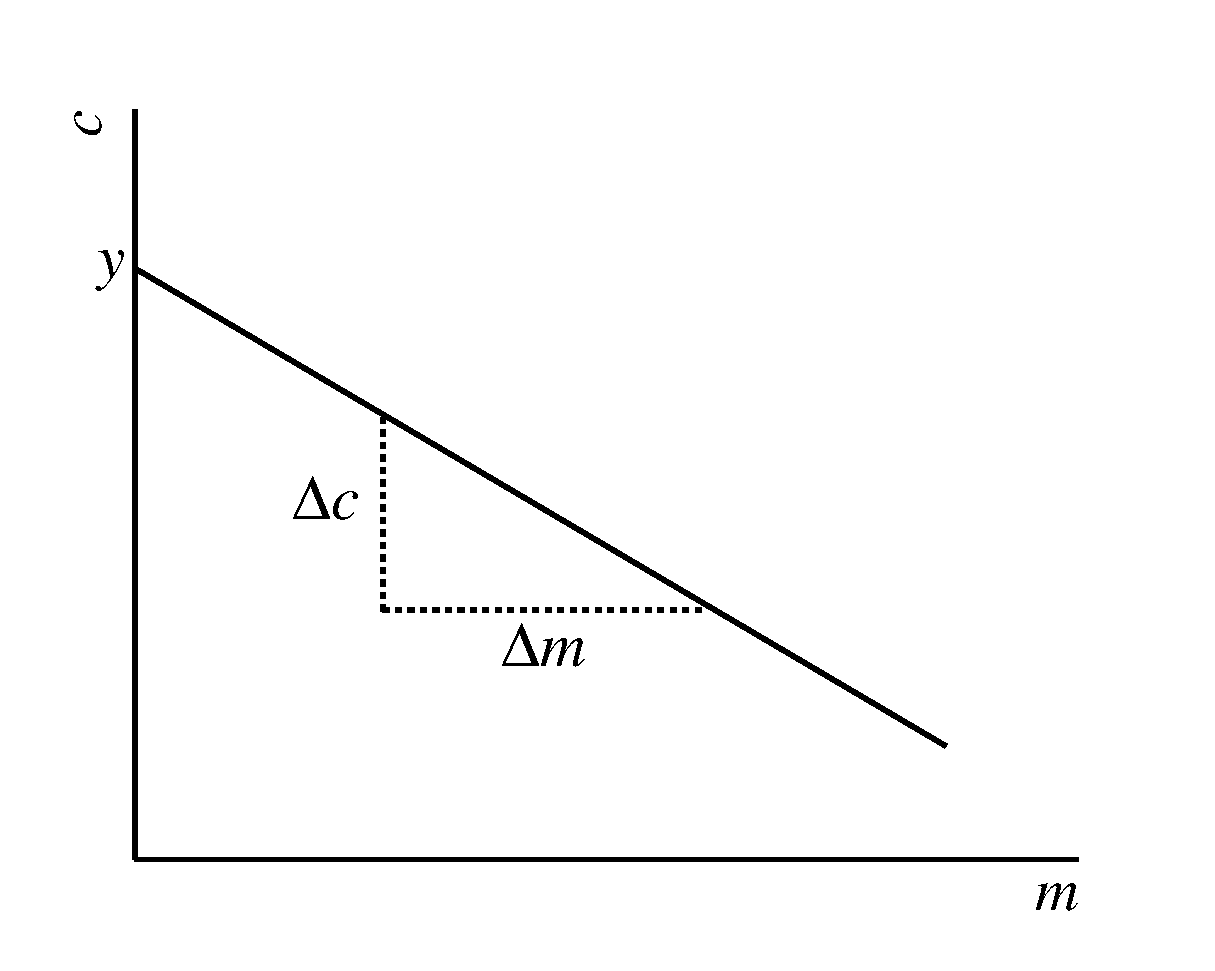
\includegraphics[width=7cm]{images/hough_transform/parameter_line} \label{fig:2DParameterLine}}
  \caption{Representations of a 2D point in Cartesian space.}
  \label{fig:2DCartesianPointAndParameterLine}
\end{figure}


\subsection{The parameter space}
\label{subsec:ParameterSpace}
As section~\ref{subsec:LinePointDuality} shows, there is a clear relationship between the Cartesian space and the parameter space.  Specifically, there is a symmetry between lines and points contained in the two spaces.  This relationship between the Cartesian and parameter spaces is not only interesting but also very powerful.  Consider again the parameter line defined by equation~\ref{eq:2DLineParameter} and shown in Fig.~\ref{fig:2DParameterLine}.  As shown in section~\ref{subsec:LinePointDuality}, equation~\ref{eq:2DLineParameter} was derived by considering the infinite set of lines which pass through a Cartesian point.  As this infinite set represents the parameter line, it must also be true that the parameter line represents the infinite line set.  Using one of the results from section~\ref{subsec:LinePointDuality}, any point along the parameter line represents one of the lines from our infinite set.  This key feature of the parameter space is the central component of the Hough transform.  
\newline
\newline
We will now return to the Cartesian space for an example of how the Hough transform works.  \YoshiFinal{Let us}{ADDRESSED - was `let's'} define three points in this space,
\begin{equation}
  \begin{split}
    &\quad p_{1}: (2,6) \\
    &\quad p_{2}: (4,8) \\
    &\quad p_{3}: (6,10).
  \end{split}
  \label{eq:HTExampleCartesianPoints}
\end{equation}
\begin{figure}%
  \centering
  \subfloat[The three Cartesian points defined in equation~\ref{eq:HTExampleCartesianPoints} along with example lines from each point's infinite line set.  The coordinates of each point are also shown.]{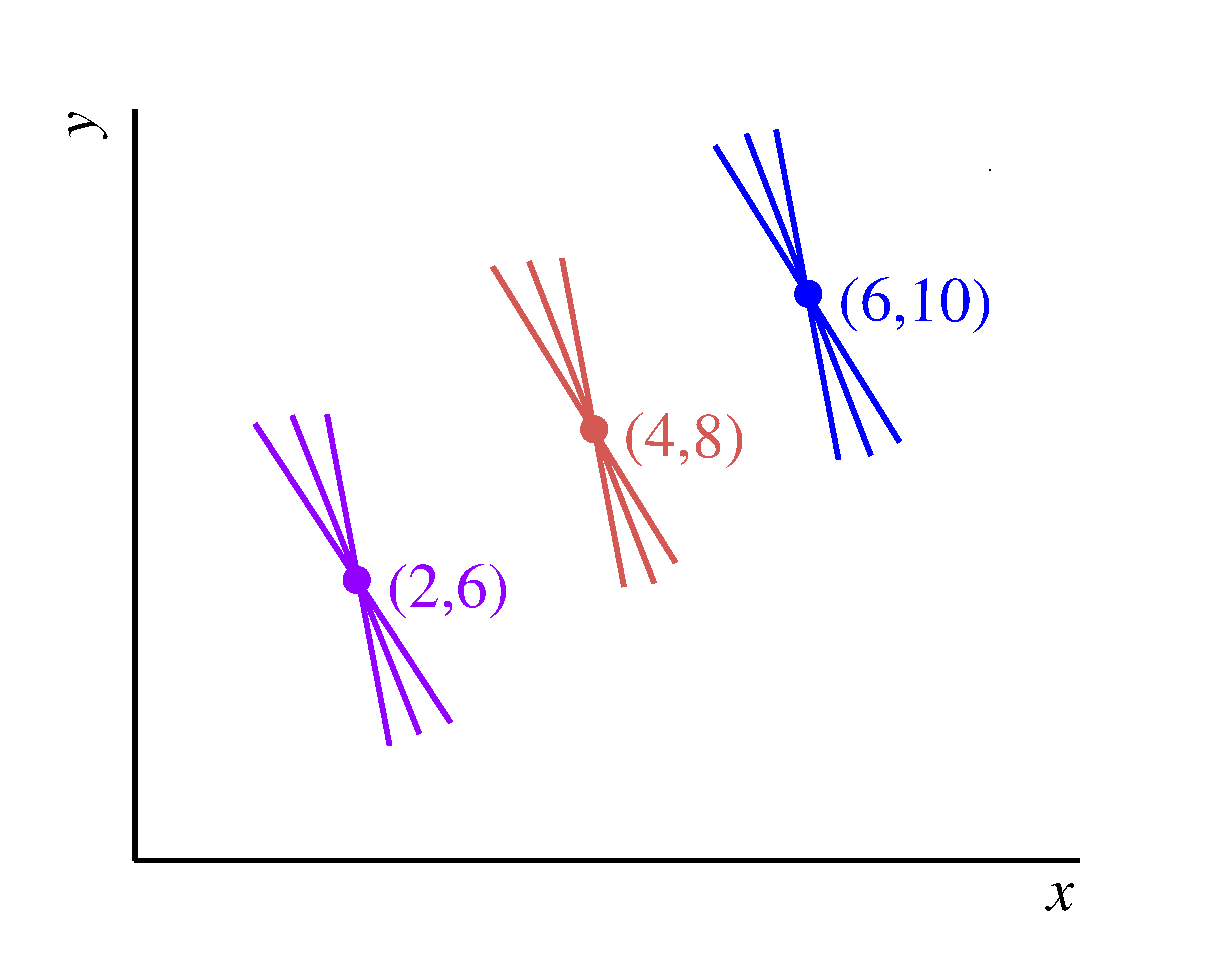
\includegraphics[width=7cm]{images/hough_transform/HT_example_cartesian_space} \label{fig:HTExampleCartesianSpace}} 
  \hspace{1em}
  \subfloat[The three parameter lines defined in equation~\ref{eq:HTExampleParameterLines}.  The coordinates (2, 4) define the point of intersection of the three lines.]{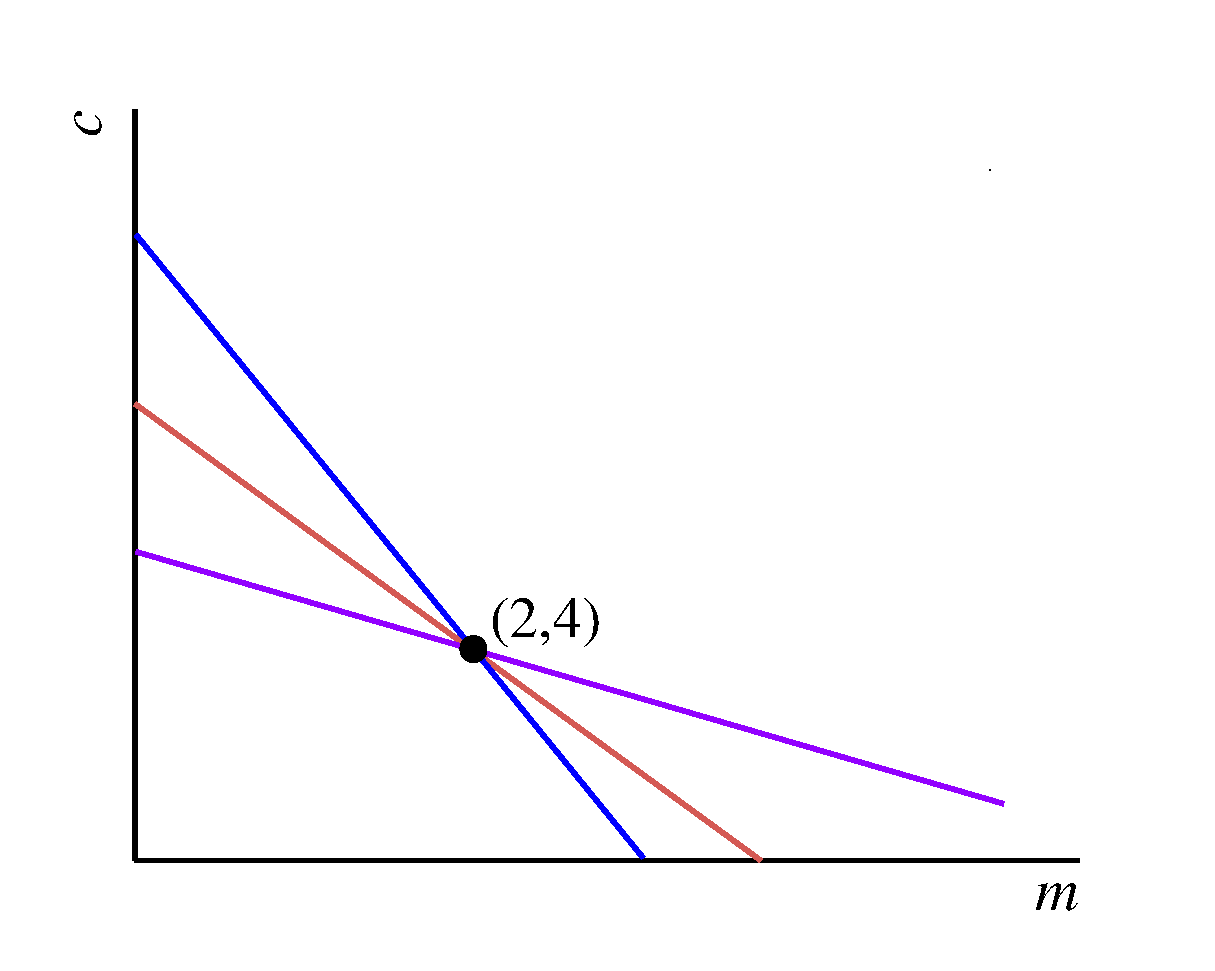
\includegraphics[width=7cm]{images/hough_transform/HT_example_parameter_space} \label{fig:HTExampleParameterSpace}}
  \caption{The three points defined in equation~\ref{eq:HTExampleCartesianPoints} and their representation in the parameter space.  The colour coding matches the Cartesian points to their respective parameter lines.}
  \label{fig:HTExample}
\end{figure}
\newline
\newline
The three points defined in equation~\ref{eq:HTExampleCartesianPoints} are shown in Fig.~\ref{fig:HTExampleCartesianSpace}.  Using one of the results from section~\ref{subsec:LinePointDuality} and equation~\ref{eq:2DLineParameter}, the three points can be Hough-transformed into the following parameter lines:
\begin{equation}
  \begin{split}
    &\quad c = -2m + 6 \\
    &\quad c = -4m + 8 \\
    &\quad c = -6m + 10.
  \end{split}
  \label{eq:HTExampleParameterLines}
\end{equation}
The three parameter lines are shown in Fig.~\ref{fig:HTExampleParameterSpace}.  From Fig.~\ref{fig:HTExampleParameterSpace}, it is clear that the three parameter lines all cross at a common point with parameter space coordinates (2, 4).  Using the results from section~\ref{subsec:LinePointDuality}, this common point in parameter space is represented by a line in Cartesian space.  In addition, as (2, 4) is common to all three parameter lines, the Cartesian line represented by (2, 4) must also pass through all three Cartesian points defined by equation ~\ref{eq:HTExampleCartesianPoints}.  This new Cartesian line is defined by
\begin{equation}
  y = 2x + 4
  \label{eq:HTExampleCartesianLine}
\end{equation}
and is shown in Fig.~\ref{fig:HTExampleCartesianSpaceWithLine} with the original points used to generate the parameter lines.  While this example is relatively simple, it demonstrates the capability of the Hough transform to recognise linear patterns in sets of points.

\begin{figure}
  \centering
  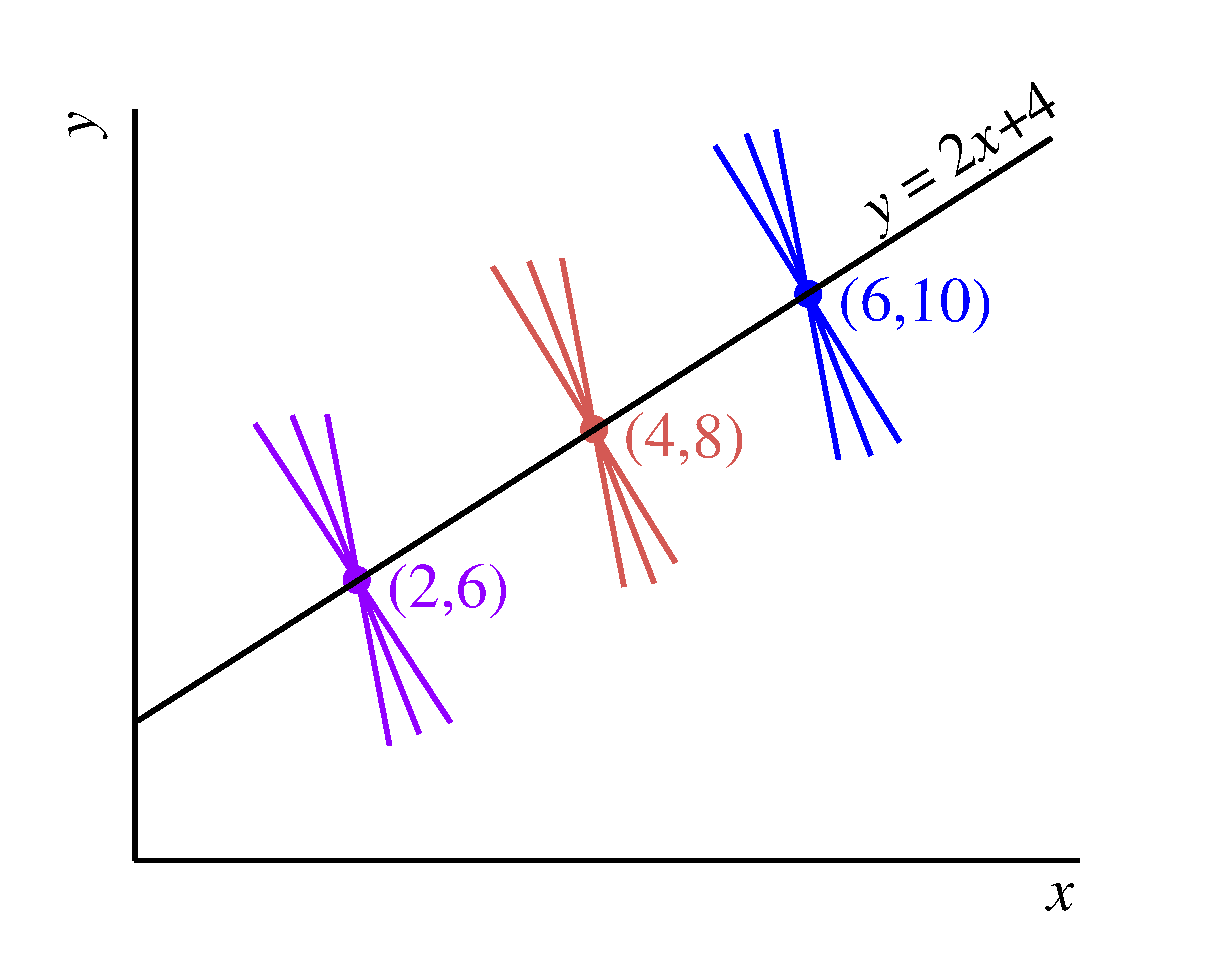
\includegraphics[width=9cm]{images/hough_transform/HT_example_cartesian_space_with_line}
  \caption{The line represented by the parameter space intersection in Fig.~\ref{fig:HTExampleParameterSpace} with the Cartesian points it intercepts.}
  \label{fig:HTExampleCartesianSpaceWithLine}
\end{figure}

\subsection{Redefinition of parameters}
\label{subsec:ParameterRedefinition}
Unfortunately, a complication in computation arises when $m\rightarrow\infty$.  However, this complication can be removed by redefining the line parameters.  An alternative 2D line parameterisation is to specify a line in terms of the angle it makes with the $x$ axis, $\theta$, and the perpendicular distance of the line from the origin, $\rho$, as illustrated in Fig.~\ref{fig:CartesianParameterRedefinition}.  The functional form of the Cartesian line becomes 
\begin{equation}
  y = x\tan\theta + \frac{\rho}{\cos\theta}.
  \label{eq:CartesianLineReparameterisation}
\end{equation}
Using this new parameterisation, we must also define a new parameter space with axes $\theta$ and $\rho$.  Using equation~\ref{eq:CartesianLineReparameterisation}, a line in this new parameter space is defined by
\begin{equation}
  \rho = y\cos\theta - x\sin\theta.
  \label{eq:ParameterLineReparameterisation}
\end{equation}
By definition, the $\theta$ axis of the parameter space must be bounded to the interval [0, 2$\pi$].  If the directionality of the line is meaningless to the analyser, then the interval can be restricted to [0, $\textrm{\pi}$].
\newline
\newline
The disadvantage of this parameterisation is that parameter line generation now involves trigonometric calculations which can be computationally expensive.  However, this problem is small when compared to the unbounded complication of the traditional parameterisation.

\begin{figure}
  \centering
  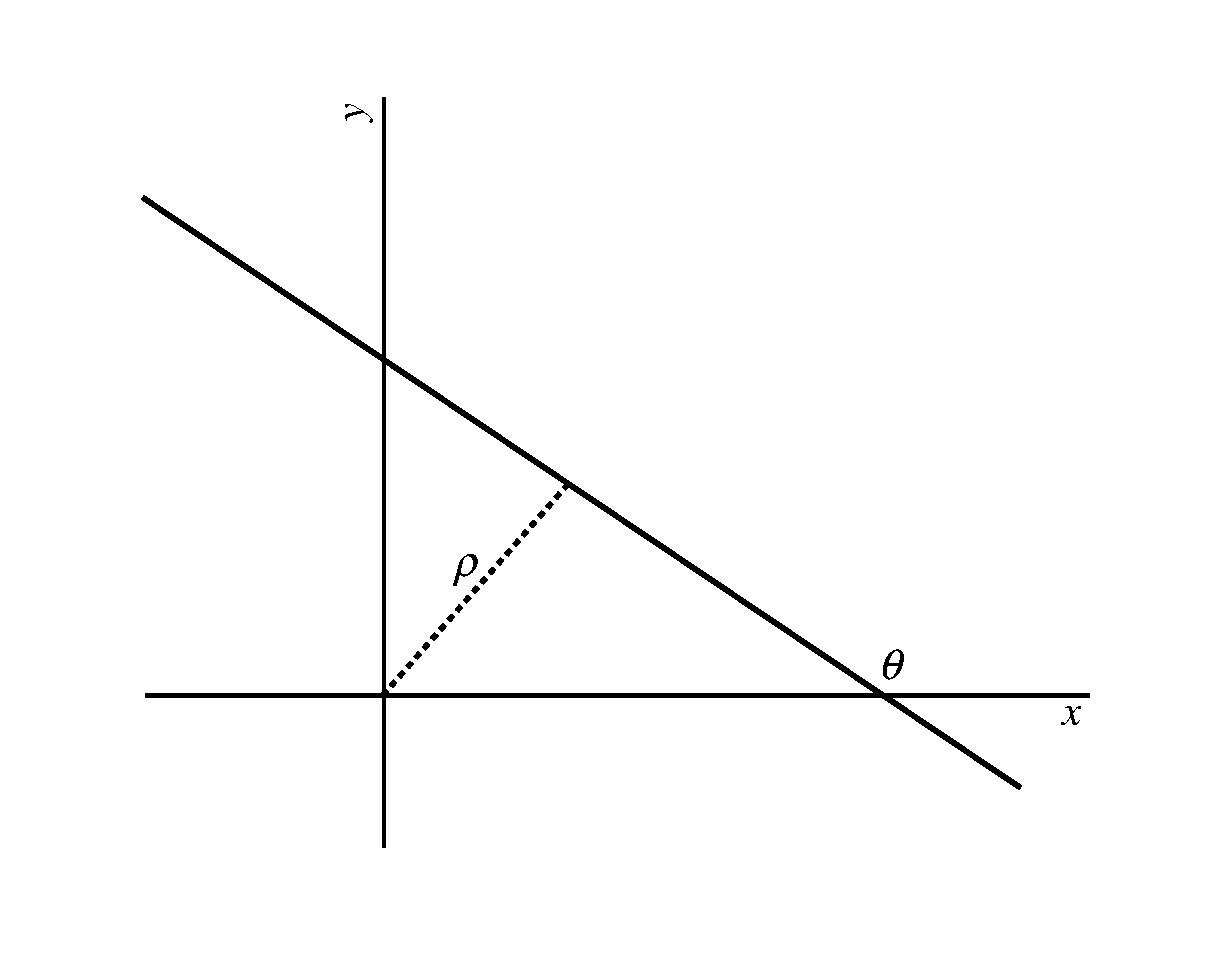
\includegraphics[width=9cm]{images/hough_transform/cartesian_parameter_redefinition}
  \caption{$\theta$-$\rho$ parameterisation of a 2D line.}
  \label{fig:CartesianParameterRedefinition}
\end{figure}



\subsection{Discretisation of the parameter space}
\label{subsec:ParameterSpaceDiscretisation}
It must now be considered how the parameter space is analysed.  When a large number of parameter lines are generated, it becomes computationally expensive to analyse the resultant parameter space.  While approaches exist to analyse the parameter space with very high precision~\cite{331821}, it is often only necessary to extract parameters with finite resolution.  In such a case, it is convenient to discretise the parameter space.  Under this regime, the parameter space is split into $\theta$-$\rho$ bins.  Then, a parameter line is generated by incrementing the value of each $\theta$-$\rho$ bin it passes through.  After each line has been added to the parameter space, the crossing locations can be readily found by searching for the $\theta$-$\rho$ bins with content larger than unity.  An example of this discretisation is illustrated in Fig.~\ref{fig:BinnedParameterSpace}, where the parameter lines defined in equation~\ref{eq:HTExampleParameterLines} have been re-parameterised using equation~\ref{eq:ParameterLineReparameterisation}.  The content of each bin in Fig.~\ref{fig:BinnedParameterSpace} records how many of the three parameter lines pass through each bin.  The bin with value 3 is the crossing point of the three parameter lines.
\newline
\newline
If a discretised approach is acceptable, which is the case in event reconstruction, construction and analysis of the parameter space is reduced to filling a 1D array $N$ times, where $N$ is the number of parameter lines, followed by a 1D grid search of the array to find the bin with the highest content.
\begin{figure}
  \centering
  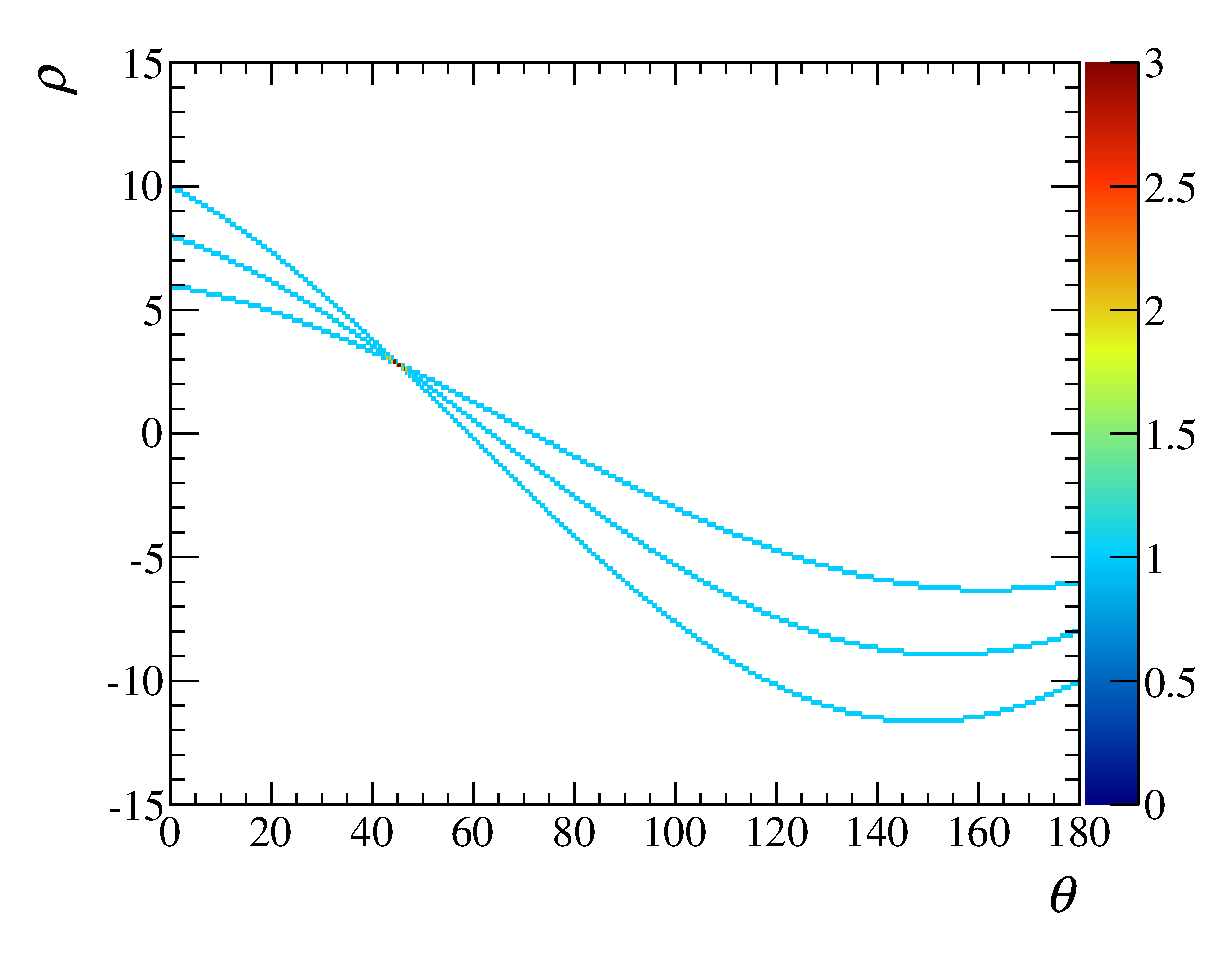
\includegraphics[width=9cm]{images/hough_transform/binned_parameter_space}
  \caption{The discrete $\theta$-$\rho$ space.  The plotted lines are those defined in equation~\ref{eq:HTExampleParameterLines} and reparameterised using equation~\ref{eq:ParameterLineReparameterisation}.}
  \label{fig:BinnedParameterSpace}
\end{figure}



\section{ECal application of the Hough transform}
\label{sec:ECalApplicationHoughTransform}
We must now address how the Hough transform can be used as a reconstruction tool in the ECal.  To do this, \YoshiFinal{let us}{ADDRESS - was `let's'} consider a neutrino interaction which occurs in the ECal as illustrated in~\ref{fig:3StateInteractionNoReconstruction}.  While the propagating neutrino is invisible to the ECal, the charged final state are definitely not.  To first order, the final state particles propagate in straight lines depositing energy in the scintillator bars as they go.  From this, we can infer that the hit bars arranged in straight lines should reveal the trajectory of the final states.  As shown above, the Hough transform is capable of identifying straight lines from a set of coordinates.  However, there are two complications in the ECal which the above sections have not addressed.  We have only specifically discussed how to extract a single straight line from a pattern.  As Fig.~\ref{fig:3StateInteractionNoReconstruction} shows, the number of final states can be, and is often, greater than one.  This is merely a problem of computation which will be addressed in section~\ref{subsec:ParameterSpaceAnalysis}.  A much more severe problem is that the above demonstrations only deal with patterns constructed from infinitesimal points.  While the centre of a scintillator bar can be used as a point for parameter line generation, it is unlikely that a final state particle will pass through the central point of the scintillator bars that it propagates through.  If this is not addressed, the Hough transform will be of little use in trajectory reconstruction.
\begin{figure}
  \centering
  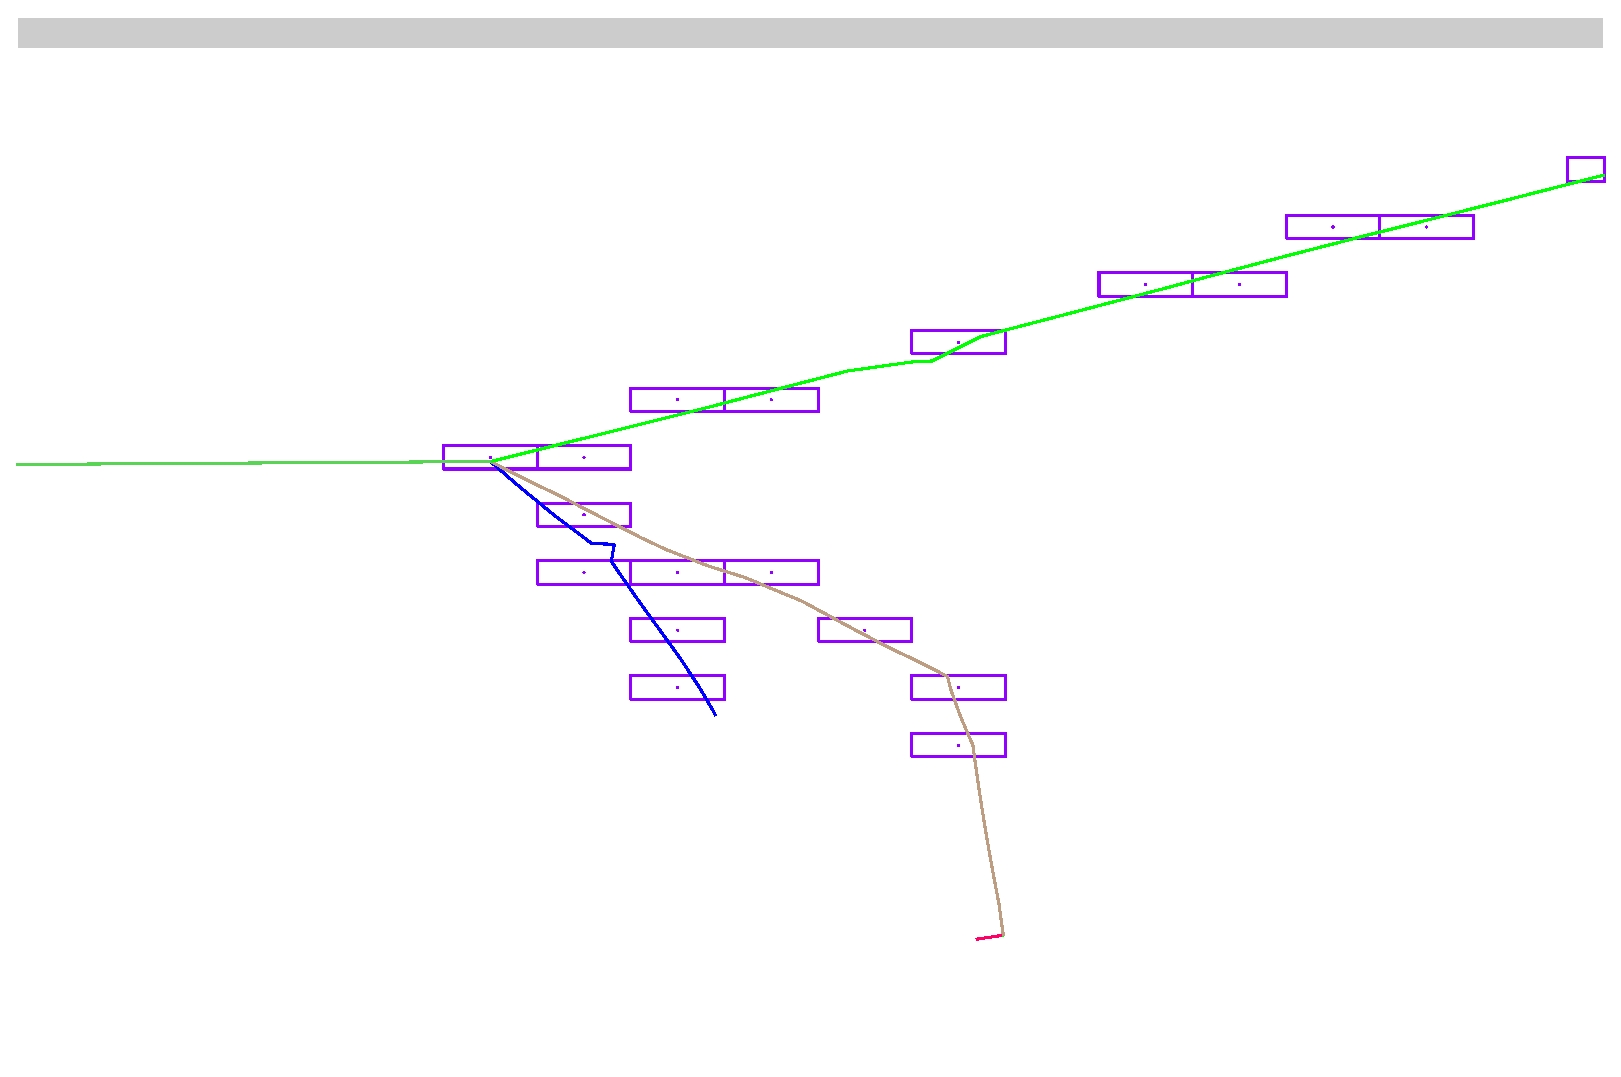
\includegraphics[width=10cm]{images/hough_transform/3StateInteraction_SideLeftECal_NoReconstruction.eps}
  \caption{Simulated neutrino interaction with 3 final states in the side-right ECal.  The green line entering from the left is the $\nu_\mu$.  The green line exiting to the right is a $\mu^{-}$, the brown line is a $\pi^+$ and the blue line is a proton.  The purple rectangles represent the hit ECal bars.}
  \label{fig:3StateInteractionNoReconstruction}
\end{figure}

\subsection{Modelling the ECal bar}
\label{subsec:ECalBarModel}
To make the Hough transform viable as a reconstruction tool, the finite dimensions of the ECal bar need to be incorporated into the parameter space generation.  This feature of the ECal bars would be very problematic if the parameter space was continuous.  However, it is only necessary to know the line parameters with finite resolution and a discrete parameter space can be used.  This means that the ECal bar can be modelled as a set of Cartesian points and each of said points can be Hough-transformed in turn to build up the parameter line representation of the ECal bar.
\newline
\newline
There are now two steps to consider.  Firstly, how should the points be arranged?  Remember that the Hough transform of a point represents all of the lines that pass through that point.  So, the points should be arranged in such a fashion that any line which passes through the 2D cross-section of the ECal bar also has to pass through one of the points in the configuration.  Secondly, the spacings between the points should be small enough that no gaps appear in the generated parameter line.  
\newline
\newline
Assuming that every bin of the parameter space will have a 1$^\circ\times$1 mm area, an obvious choice would be to use a rectangular grid of points with 1 mm spacing superimposed over the 2D cross-section of an ECal bar.  The total number of points used to model the ECal bar is 451.  To Hough transform the ECal bar, every point in the grid array can be Hough-transformed individually with care taken to ensure that each $\theta-\rho$ bin is filled exactly once.  The result is illustrated in Fig.~\ref{fig:ECalBarHoughTransformGridRepresentation}.  The finite size of the ECal bar is evident by the finite size of the resultant parameter line.
\begin{figure}%
  \centering
  \subfloat[Grid representation of an ECal bar.]{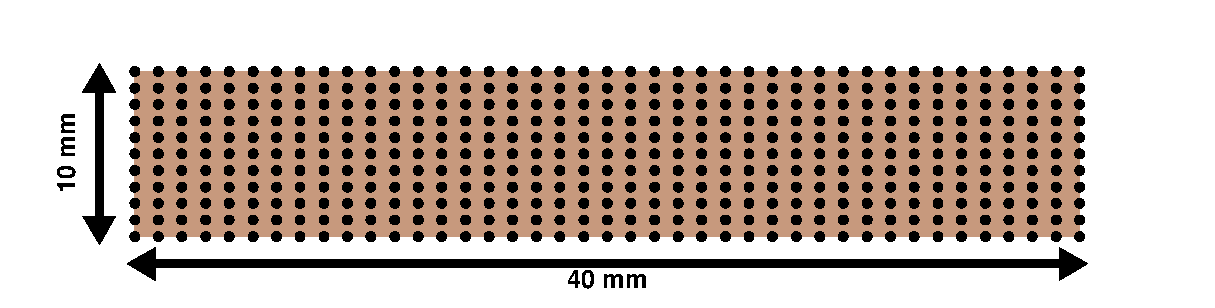
\includegraphics[width=7cm]{images/ecal_hough_transform/ecal_grid_array.eps} \label{fig:ECalBarGridRepresentation}}
  \hspace{1em}
  \subfloat[Single ECal bar Hough transform using the point configuration shown in Fig.~\ref{fig:ECalBarGridRepresentation}.]{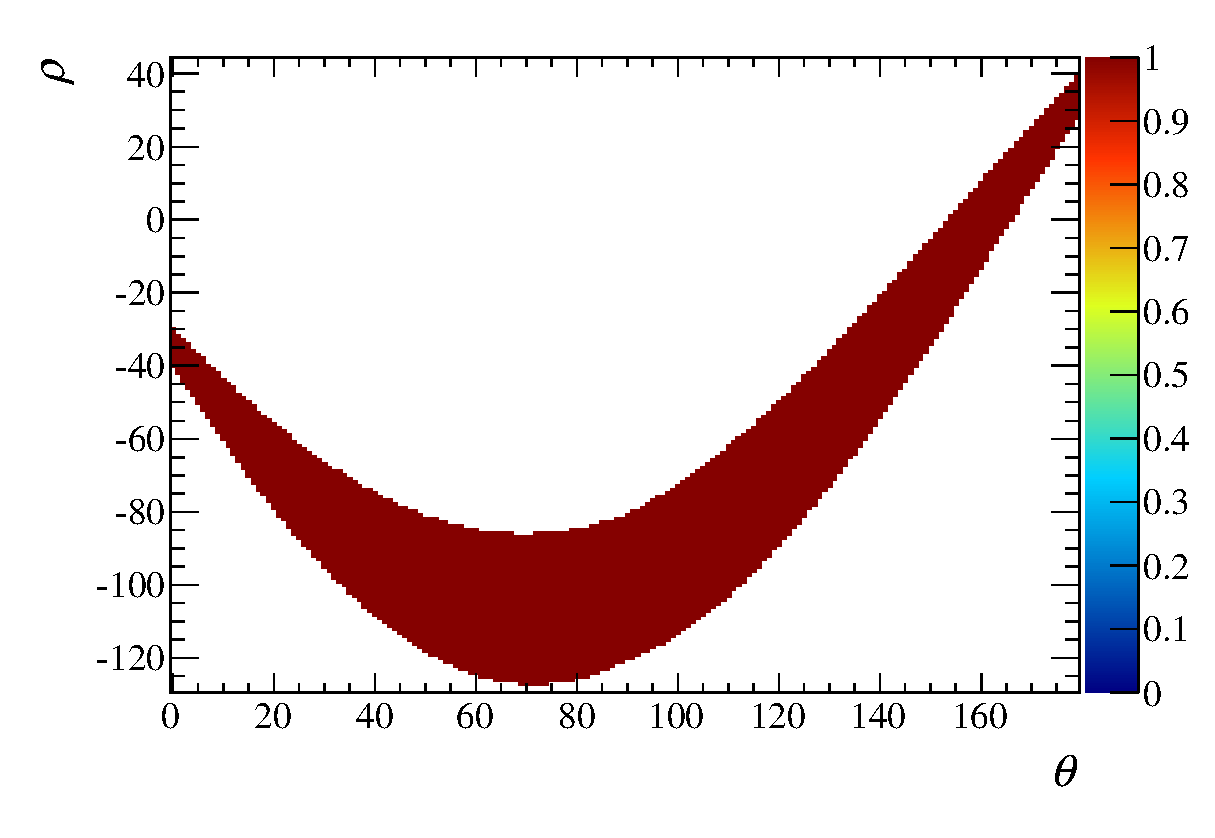
\includegraphics[width=7cm]{images/ecal_hough_transform/single_ecal_bar_hough_transform.eps} \label{fig:ECalBarHoughTransformGridRepresentation}}
  \caption{The grid representation of an ECal bar and its representation in parameter space.}
  \label{fig:ECalBarGridRepresentationAndHoughTransform}
\end{figure}
\newline
\newline
While the generated parameter line accurately represents every line which passes through the ECal bar, there are two problems with this approach.  Firstly, the large number of points to be Hough-transformed is very large which results in a long CPU time.  Secondly, there is a very high number of redundant calculations involved in the parameter line generation.  Consider an exactly vertical line which passes through one of the points in the grid array.  This line also passes through 10 other points in the same column of the grid.  This means that when the parameter line is being generated, this vertical line is calculated 11 times for each column.  Bearing this in mind, there are many points along the parameter line which are repeatedly calculated and provide no extra information.  This would mean that any algorithm which uses this approach would be very CPU inefficient.
\newline
\newline
An alternative is to model the ECal bar as a set of points arranged in a cross as shown in Fig.~\ref{fig:ECalBarCrossRepresentation}.  Assuming that the spacing between the points on each line of the cross is infinitesimal, any line which passes through the ECal bar would also have to pass through one of the points in the configuration.  As the parameter space is discrete, the spacing between the points need not be infinitesimal but only small enough to ensure that no gaps appear in the parameter line.  Using 45 points on each line of the cross, the ECal bar can be Hough-transformed by \YoshiFinal{Hough-}{ADDRESSED - was `Hough': There can be too many Houghs in a sentence}transforming each point in the cross configuration. An example of this result is shown in Fig.~\ref{fig:ECalBarHoughTransformCrossRepresentation} using the same ECal bar used to generate Fig.~\ref{fig:ECalBarHoughTransformGridRepresentation}.  Clearly, Fig.~\ref{fig:ECalBarHoughTransformGridRepresentation} and Fig.~\ref{fig:ECalBarHoughTransformCrossRepresentation} are identical showing that the cross model achieves the same result as the grid model.  Comparing the two, the cross model uses a 90 point representation whereas the grid model uses a 451 point representation.  This should mean that an algorithm utilising the cross model would be a factor of five faster than one using a grid model.
\begin{figure}%
  \centering
  \subfloat[Cross representation of an ECal bar.]{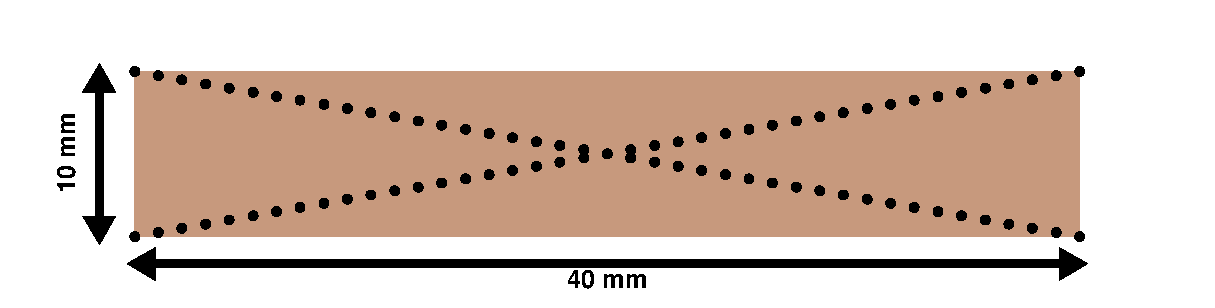
\includegraphics[width=7cm]{images/ecal_hough_transform/ecal_cross_array.eps} \label{fig:ECalBarCrossRepresentation}}
  \hspace{1em}
  \subfloat[Single ECal bar Hough transform using the point configuration shown in Fig.~\ref{fig:ECalBarCrossRepresentation}.]{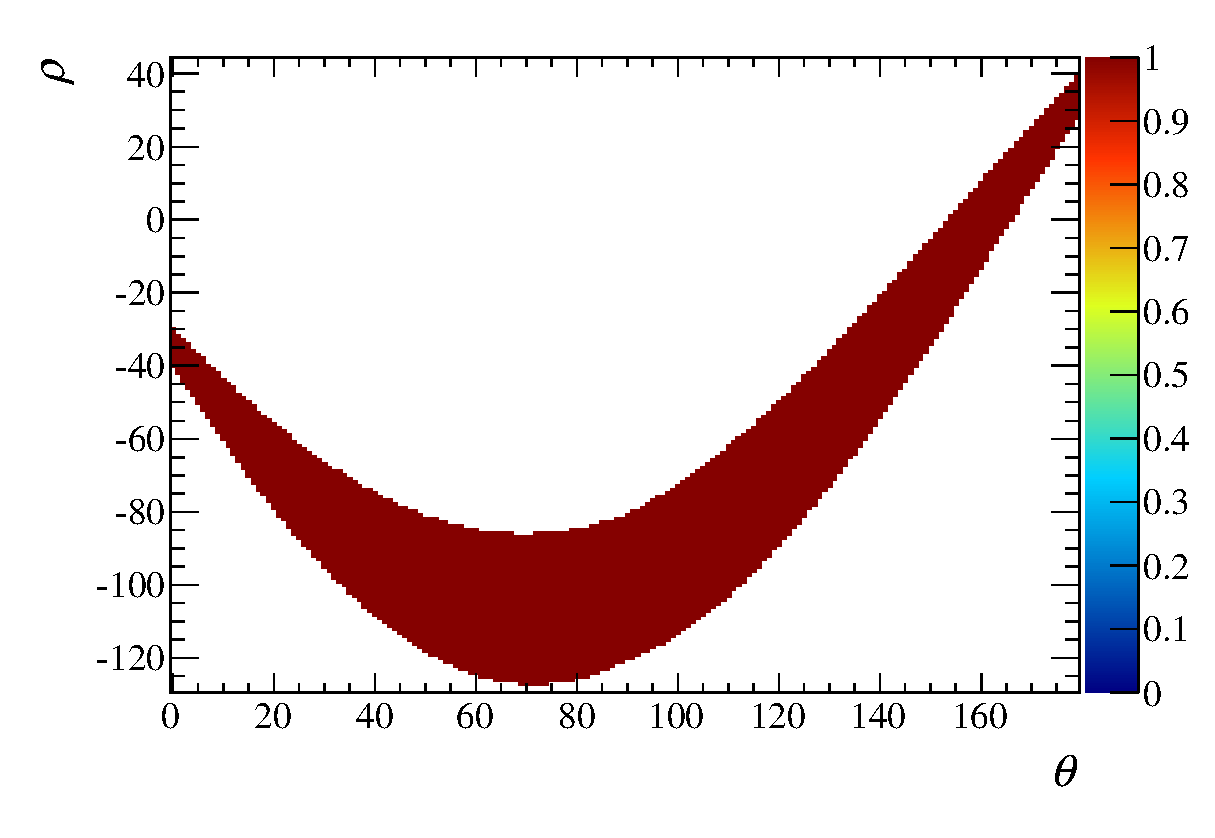
\includegraphics[width=7cm]{images/ecal_hough_transform/single_ecal_bar_hough_transform.eps} \label{fig:ECalBarHoughTransformCrossRepresentation}}
  \caption{The cross representation of an ECal bar and its representation in parameter space.}
  \label{fig:ECalBarCrossRepresentationAndHoughTransform}
\end{figure}

\subsection{Parameter space generation}
\label{subsec:ParameterSpaceGeneration}
As we have addressed how to Hough-transform an ECal bar, we are now in suitable position to generate the full parameter space for an ECal cluster.  As described in section~\ref{subsec:ParameterRedefinition}, the parameterisation of the 2D lines requires some point in space to act as the origin.  It is possible to use the origin defined by the global ND280 geometry\Yoshi{; however,}{ADDRESSED - was ``, however''} this is located in TPC 1 which would mean $\rho$ will usually be \YoshiFinal{of}{ADDRESSED - } the order of metres.  It is more convenient to define an origin in the vicinity of the ECal cluster being reconstructed.  A simple option is to use the charge-weighted centre of the ECal cluster as the origin of the Hough transform.  This location is simple to calculate and generally keeps $\rho$ small.
\newline
\newline
The provided description of the Hough transform in all previous sections is strictly defined in 2D and so the ECal cluster should be split in such a way that this definition can be used.  Fortunately, a 3D ECal cluster is built up using the two 2D views that the scintillator layers provide.  So, it is relatively easy to split the 3D cluster into a pair of 2D clusters by collecting the cluster's hits into their respective 2D views.
\newline
\newline
We can now partly answer one of the problems raised in section~\ref{sec:ECalApplicationHoughTransform} which is how to handle the track multiplicity aspect of the reconstruction\YoshiFinal{.}{ADDRESSED - was `?', but it isn't actually a question} This is partly addressed by generating $N$ parameter spaces with the same $\theta$-$\rho$ bin configuration where $N$ is the number of hits in the 2D cluster.  Each of the $N$ parameter spaces will hold one parameter line generated by one of the 2D hits (in a similar fashion to Fig.~\ref{fig:ECalBarHoughTransformCrossRepresentation}).  The final parameter space can then be generated by adding together each of the $N$ parameter spaces.  The parameter space of the 2D cluster in Fig~\ref{fig:3StateInteractionNoReconstruction} is shown in Fig.~\ref{fig:FullParameterSpace3StateInteraction}.
\begin{figure}
  \centering
  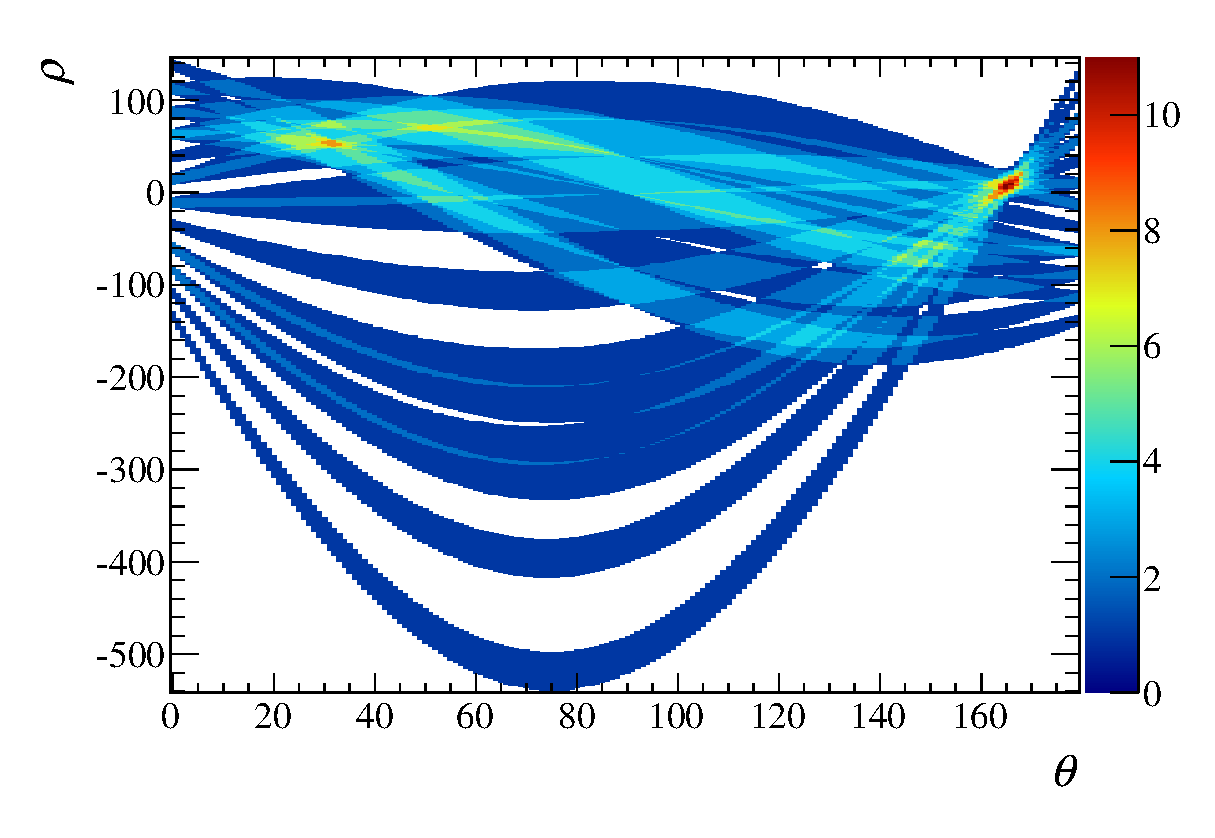
\includegraphics[width=10cm]{images/ecal_hough_transform/FullParameterSpace_3StateInteraction.eps}
  \caption{The full parameter space of the 2D cluster shown in Fig.~\ref{fig:3StateInteractionNoReconstruction}.  The height of each point in the parameter space corresponds to the number of hit scintillator bars intersected by the Cartesian line which the parameter space point represents.}
  \label{fig:FullParameterSpace3StateInteraction}
\end{figure}


\subsection{Parameter space analysis}
\label{subsec:ParameterSpaceAnalysis}
The full parameter space can look arbitrarily complicated. However, it contains a vast amount of trajectory related information about the cluster.  Every $\theta$-$\rho$ bin of the parameter space describes a 2D track and the content value of said bin describes how many 2D ECal hits the track passes through.  As described in section~\ref{sec:ECalApplicationHoughTransform}, a particle's trajectory should be straight in the ECal which means that the particles path should be revealed by finding the most hits arranged in a line.  This hit arrangement can be found by finding the bin in the full parameter space with the highest value.  The track candidate parameters can the be found by fetching the ($\theta$, $\rho$) coordinate of the found bin.
\newline
\newline
While the preferred bin can reveal how many hits the track candidate passed through, it contains no information about which hits were contributors.  However, this full parameter space was generated by summing the $N$ parameter spaces discussed in section~\ref{subsec:ParameterSpaceGeneration}.  So, the contributing hits can be readily found by looking at the same ($\theta$, $\rho$) bin in each of the $N$ parameter spaces and recording which have a non-zero value.  We now have the track candidate's parameters and its contributing hits which is enough to describe the 2D trajectory.
\newline
\newline
A new search now needs to begin to find any other track candidates.  However, repeating the same search of the full parameter space will return the track candidate that has already been found.  To find the next track candidate, the presence of the previous track candidate must be removed.  So, a reduced parameter space must be generated. The previous step found which of the $N$ parameter lines contributed to the previous track candidate.  So, this new parameter space can be formed by subtracting the contributing parameter lines from the full space.  An example of this is shown in Fig.~\ref{fig:ReducedParameterSpace3StateInteraction} where the reduced parameter space was formed by subtracting the contributing parameter lines to the highest bin in Fig.~\ref{fig:FullParameterSpace3StateInteraction}.  The next track candidate can then be found by searching for the highest content bin of this reduced parameter space and said bin's contributing parameter lines. 
\newline
\newline
This process can be repeated until some threshold is reached.  This threshold is nominally set by demanding that at least three hits are required to form a track candidate.
\begin{figure}
  \centering
  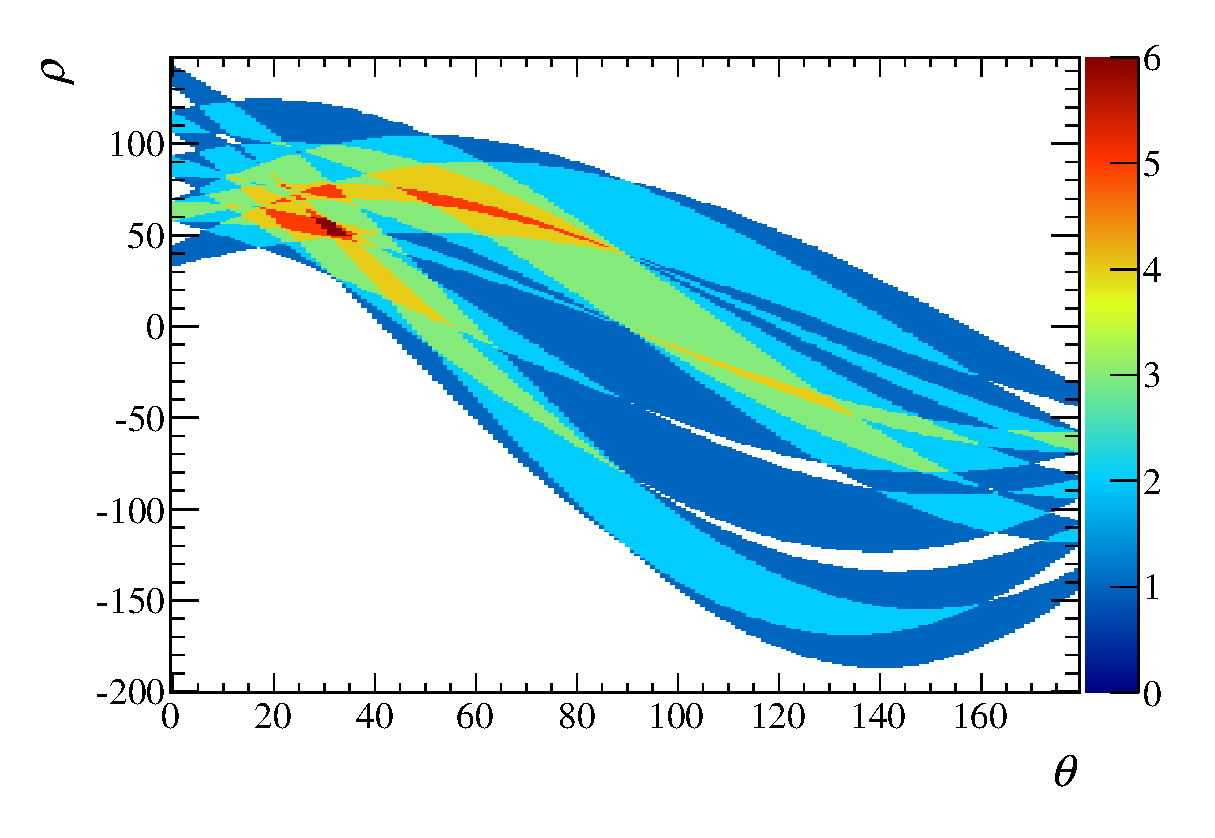
\includegraphics[width=10cm]{images/ecal_hough_transform/ReducedParameterSpace_3StateInteraction.eps}
  \caption{The reduced parameter space of the 2D cluster shown in Fig.~\ref{fig:3StateInteractionNoReconstruction}.  The reduced parameter space was formed by removing all of the hit scintillator bar representations which contributed to the full parameter space's (see Fig.~\ref{fig:FullParameterSpace3StateInteraction}) maximum.}
  \label{fig:ReducedParameterSpace3StateInteraction}
\end{figure}

\subsection{2D track quality checks}
\label{subsec:2DTrackQualityChecks}
While the approach outlined above is very powerful for recognising track-like shapes in the 2D ECal clusters, it is not capable of checking whether the selected track candidates are of sound quality.  So, external checks need to be done which validate each track as it is returned from the parameter space.  Fortunately, the objects returned from parameter space are simple in structure and so the quality checks can be designed to reflect this.  Two necessary checks were implemented in the 2D reconstruction:
\begin{itemize}
\item The track can not skip a scintillator layer in a given view.
\item The track can skip a maximum of 1 bar in a scintillator layer.
\end{itemize}
If a track fails either of the above conditions, the track is flagged as bad and rejected.  To ensure that the same bad track is not selected in the next interaction of the parameter space analysis, the track also needs removing from the parameter space.  To do this, every bin in the parameter space is checked to see if the bin is filled purely from the hits contained in the bad track.  If this is the case, the bin content is set to 0.  

\subsection{3D track reconstruction}
\label{subsec:3DHoughTrackReconstruction}
Section~\ref{subsec:ParameterSpaceAnalysis} describes the track reconstruction of a 2D ECal cluster.  However, a 3D cluster consists of two sets of 2D clusters.  So, the process described in section~\ref{subsec:ParameterSpaceAnalysis} must be performed on each of the 2D clusters.  The result of this process is two sets of 2D tracks.  To form full 3D tracks, the tracks from each view must now be matched together.  This is achieved by making every pairwise comparison of the tracks from each view to find the pair which are most similar to each other.  After such a pair is found, the tracks are removed from the pool and the process is repeated to find the next pair until either no tracks are left or one 2D track is left.  In the latter case the single 2D track is discarded. Every pairwise combination of tracks is used to form a likelihood $\mathcal{L}$.  The pair which produces the highest $\mathcal{L}$ is declared the best match and removed from the pool.  Three pieces of information about the matching pair are used to calculate $\mathcal{L}$, all of which make use of probability density distributions generated using beam Monte Carlo.  
\newline
\newline
As should be expected, a vertex with one visible track will have different characteristics to a vertex with three visible tracks.  So, to maximise the ability of the matcher, a different set of probability density distributions are used for the 1, 2 and 3 track cases.  If the number of tracks in each view is not identical, the higher number of tracks is used to find the correct probability density distributions.  Separately, due to their geometrical differences, the reconstructed shape of vertices in the DS ECal will differ to those in the barrel ECals.  This leads to a separate set of probability density distributions for the barrel and DS ECal modules.
\begin{figure}[t!]
  \centering
\Yoshi{}{ADDRESSED - Say what the reader should take away from these plots. The reader should not have to go to the body text to figure this out.}
  \subfloat[$Q_{\textrm{ratio}}$ distribution (area normalised).  The blue and red distributions refers to matching pairs which were matched to the same true particle and different true particles respectively.  The two distributions peak at different values of $Q_{\textrm{ratio}}$, which implies $Q_{\textrm{ratio}}$ provides good separation of the correctly and incorrectly matched events.]{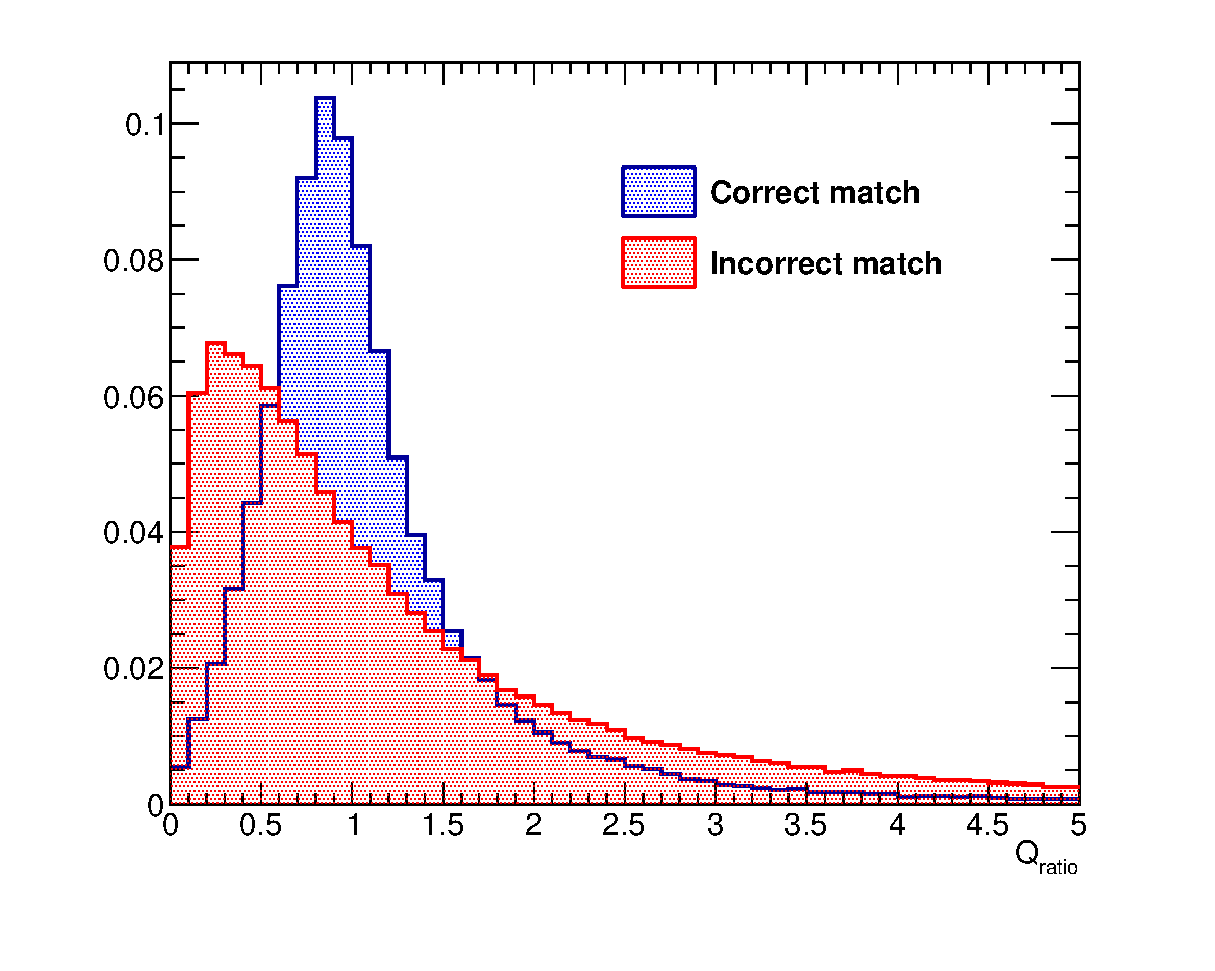
\includegraphics[width=7cm]{images/hough_3d_matching/3DMatching_Barrel_2Track_QRatio_Separation.eps} \label{fig:3DMatchingBarrel2TrackQRatioSeparation}}
  \hspace{1em}
  \subfloat[$Q_{\textrm{ratio}}$ probability density distribution.  The peak of the distribution aligns well with the correct matches peak in Fig.~\ref{fig:3DMatchingBarrel2TrackQRatioSeparation} which aides in maximising the number of correct matches made.]{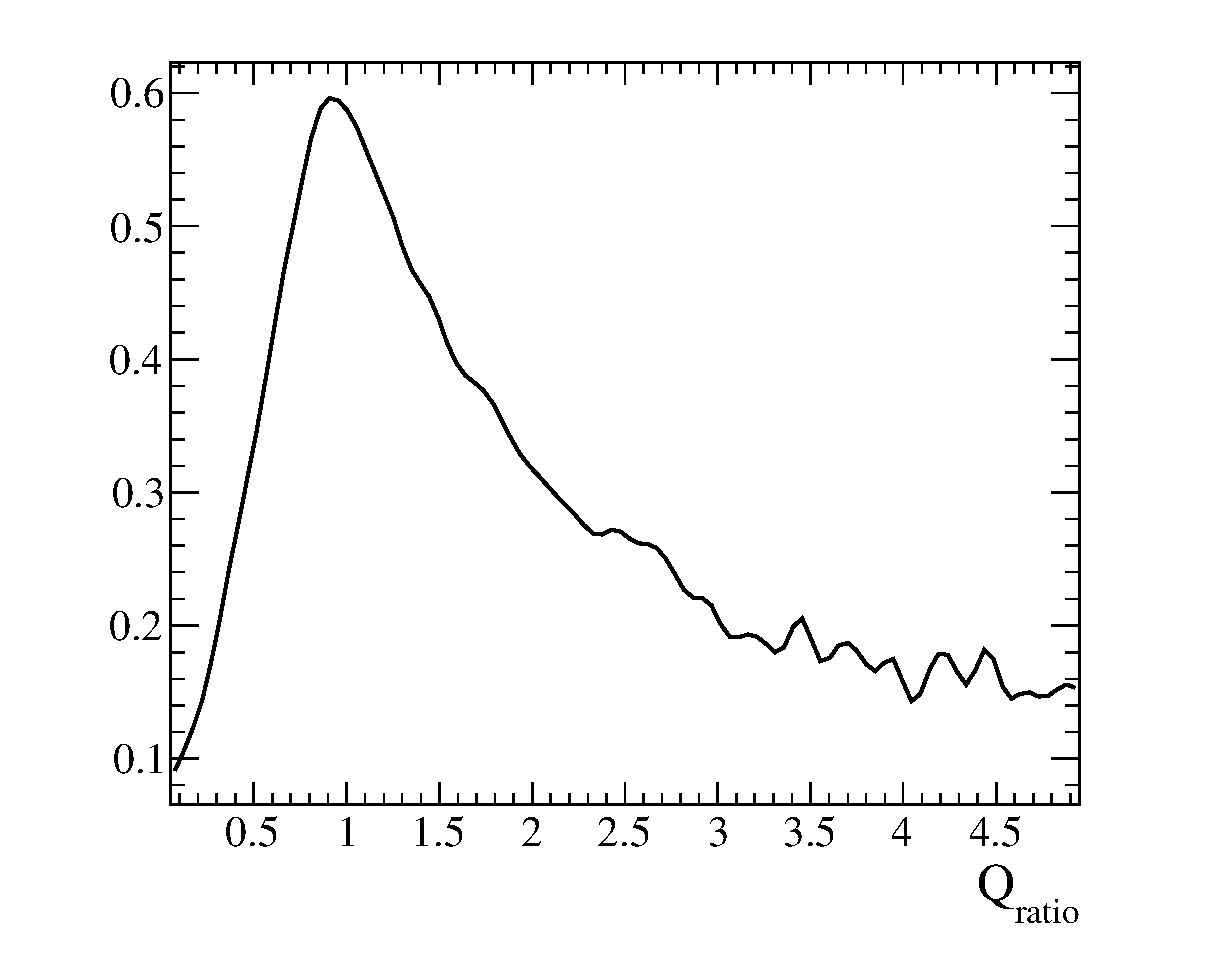
\includegraphics[width=7cm]{images/hough_3d_matching/3DMatching_Barrel_2Track_QRatio_PDF.eps} \label{fig:3DMatchingBarrel2TrackQRatioPDF}}
  \caption{$Q_{\textrm{ratio}}$ and its probability density distribution in the barrel ECal for the two track case.  NEUT-based simulation of ND280 beam events were used to produce the distributions.}
  \label{fig:QRatio}
\end{figure}
\newline
\newline
The first input to the likelihood is the ratio of the total deposited charge on each track, $Q_{\textrm{ratio}}$.  The denominator is taken as the track which comes from the view with the most hits.  Generally speaking, a particle propagating through an ECal module should deposit a similar amount of charge in each of the two views.  So, $Q_{\textrm{ratio}}$ should have a value close to 1 if the two 2D tracks are created by the same particle.  An example of the $Q_{\textrm{ratio}}$ distribution is shown in Fig.~\ref{fig:3DMatchingBarrel2TrackQRatioSeparation}, taken from beam Monte Carlo in the barrel ECals for cases where the maximum number of tracks found in a given view is 2.  In Fig.~\ref{fig:3DMatchingBarrel2TrackQRatioSeparation}, correctly matched (in blue) shows the $Q_{\textrm{ratio}}$ distribution for matching pairs which come from the same particle and incorrectly matched (in red) shows the $Q_{\textrm{ratio}}$ distribution for matching pairs which were created by different particles.  As Fig.~\ref{fig:3DMatchingBarrel2TrackQRatioSeparation} shows, $Q_{\textrm{ratio}}$ well separates the two cases.  To generate a probability density distribution for $Q_{\textrm{ratio}}$, the two distributions shown in Fig.~\ref{fig:3DMatchingBarrel2TrackQRatioSeparation} are used, but without applying any normalisation.  By comparing the bins of each distribution, the probability for correctly matching two tracks in a given bin $p_{i}$ can be formed by
\begin{equation}
  p_i = \frac{s_i}{s_i + b_i}
  \label{eq:BinProbabilityPDF},
\end{equation}
where $s_i$ is the number of correctly matched tracks in bin $i$ and $b_i$ is the number of incorrectly matched tracks in bin $i$.  A discreet probability density distribution for $Q_{\textrm{ratio}}$ can then be formed by calculating $p_i$ for every bin.  The discreet probability density distribution is then interpolated with splines to create the final probability distribution.  An example of this for the two track, barrel case is shown in Fig.~\ref{fig:3DMatchingBarrel2TrackQRatioPDF}.  When a matching candidate pair is being considered, the value of $Q_{\textrm{ratio}}$ is calculated and used in the spline to retrieve $\mathcal{L}_{Q_{\textrm{ratio}}}$.
\newline
\newline
\begin{figure}%
\Yoshi{}{Say what the reader should take away from these plots. The reader should not have to go to the body text to figure this out.}
  \centering
  \subfloat[$\Delta_{\textrm{layer, first}}$ distribution (area normalised).  The blue and red distributions refers to matching pairs which were matched to the same true particle and different true particles respectively.  While both distributions peak in the same place, the peak for the correct matches distribution is much sharper, indicating a good level of separation between the correctly and incorrectly matches events.]{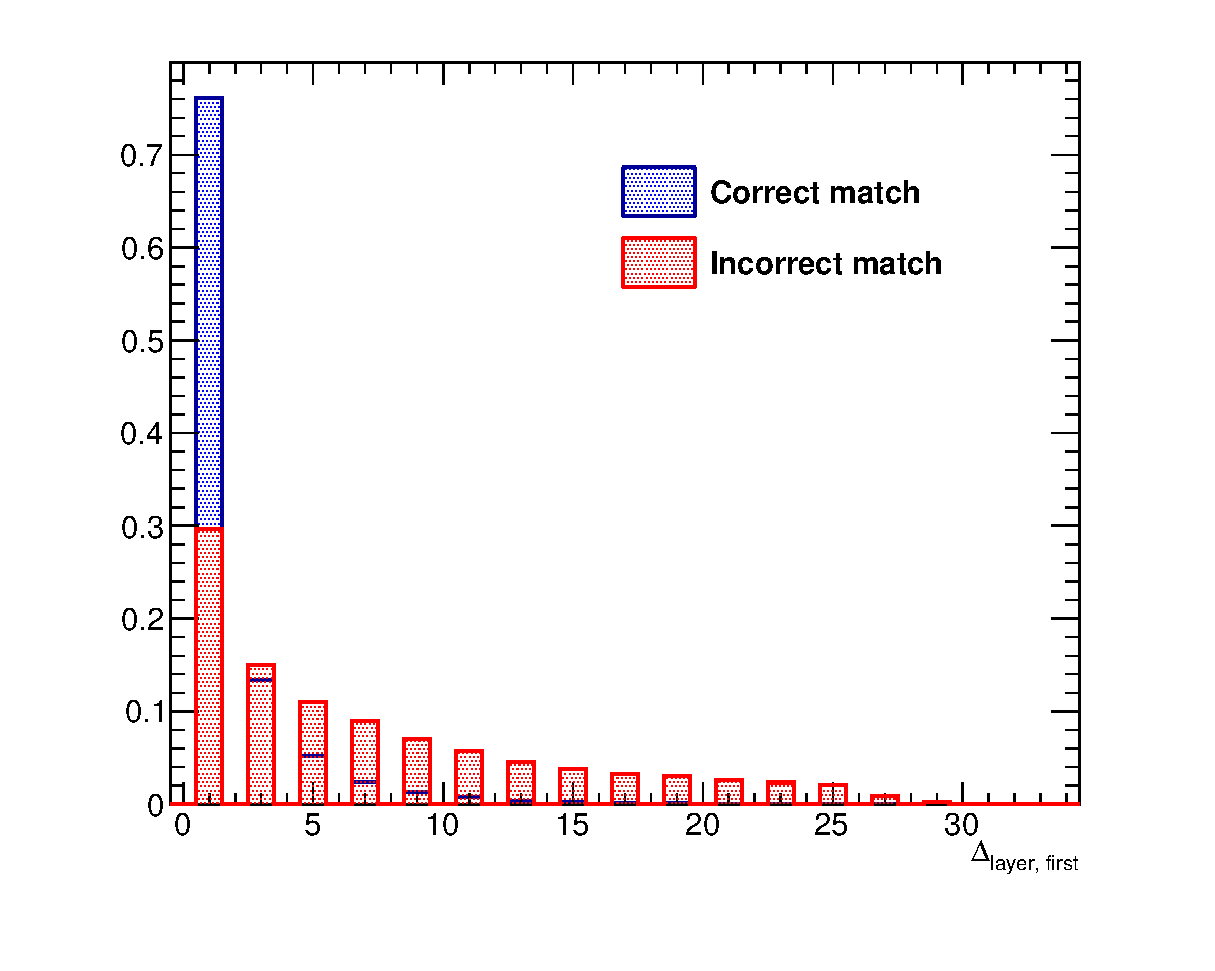
\includegraphics[width=7cm]{images/hough_3d_matching/3DMatching_Barrel_2Track_DFL_Separation.eps} \label{fig:3DMatchingBarrel2TrackDFLSeparation}}
  \hspace{1em}
  \subfloat[$\Delta_{\textrm{layer, first}}$ probability density distribution.  The peak of the distribution aligns well with the correct matches peak in Fig.~\ref{fig:3DMatchingBarrel2TrackDFLSeparation} which aides in maximising the number of correct matches made.]{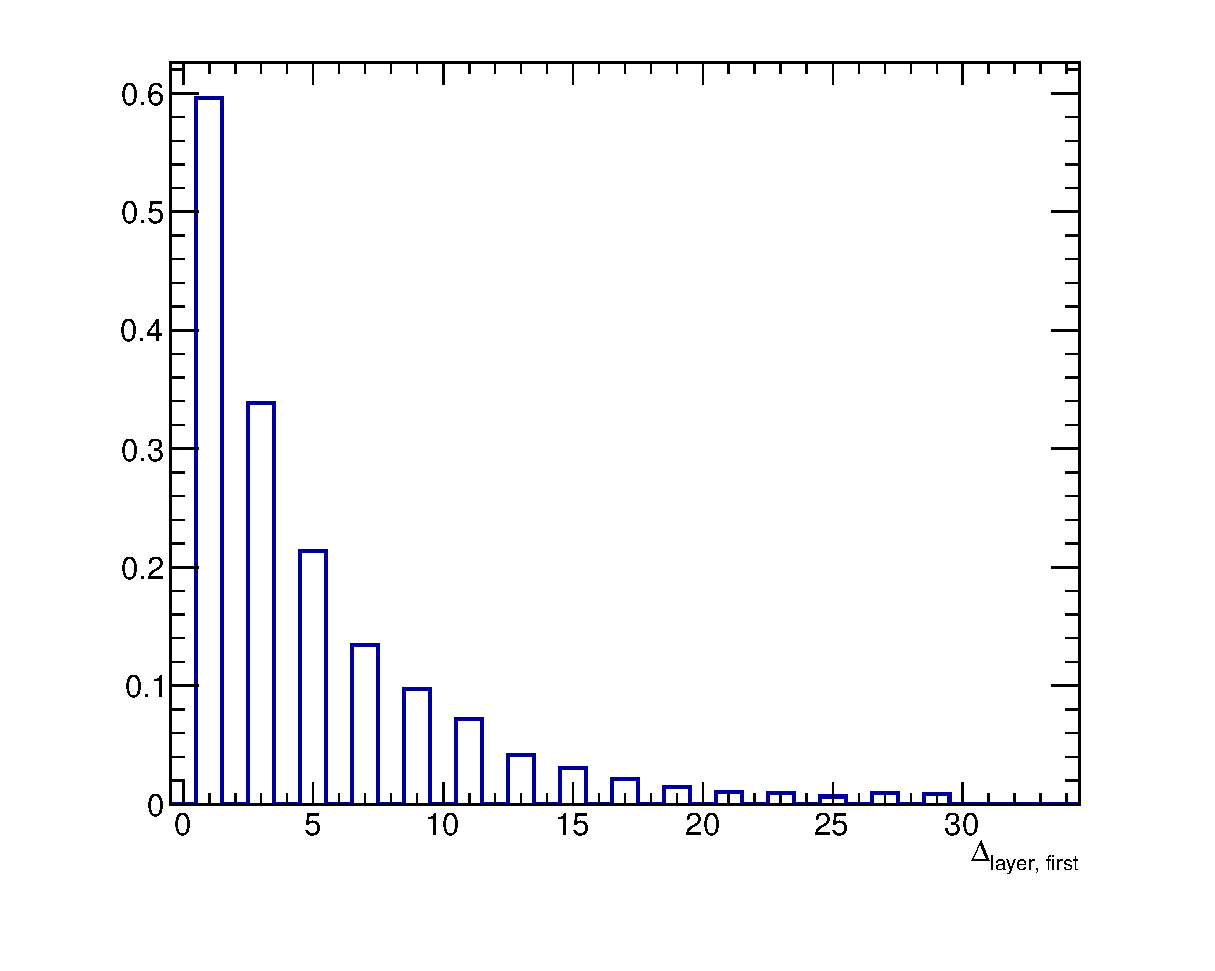
\includegraphics[width=7cm]{images/hough_3d_matching/3DMatching_Barrel_2Track_DFL_PDF.eps} \label{fig:3DMatchingBarrel2TrackDFLPDF}}
  \caption{$\Delta_{\textrm{layer, first}}$ and its probability density distribution in the barrel ECal for the two track case.  NEUT-based simulation of ND280 beam events were used to produce the distributions.}
  \label{fig:DFL}
\end{figure}
The second input to the likelihood, called $\Delta_{\textrm{layer, first}}$, is the difference in the starting layer of each 2D track which forms the matching candidate pair, where starting layer refers to the layer closest to the ND280 Tracker.  For 2D tracks which should be matched together, $\Delta_{\textrm{layer, first}}$ should be 1.  The separation ability of this variable for the two track, barrel is shown in Fig.~\ref{fig:3DMatchingBarrel2TrackDFLSeparation}.  The discreet probability density function was created using equation~\ref{eq:BinProbabilityPDF}.  It was not necessary to interpolate using splines as $\Delta_{\textrm{layer, first}}$ is itself discreet.  The probability density function for $\Delta_{\textrm{layer, first}}$ is shown in Fig.~\ref{fig:3DMatchingBarrel2TrackDFLPDF} for the two track, barrel case.  For each matching candidate pair, the value of $\Delta_{\textrm{layer, first}}$ is calculated and the corresponding $\mathcal{L}_{\Delta_{\textrm{layer, first}}}$ is retrieved from the probability density function.
\newline
\newline
\begin{figure}%
  \centering
  \subfloat[$\Delta_{\textrm{layer, last}}$ distribution (area normalised).  The blue and red distributions refers to matching pairs which were matched to the same true particle and different true particles respectively.  While both distributions peak in the same place, the peak for the correct matches distribution is much sharper, indicating a good level of separation between the correctly and incorrectly matches events.]{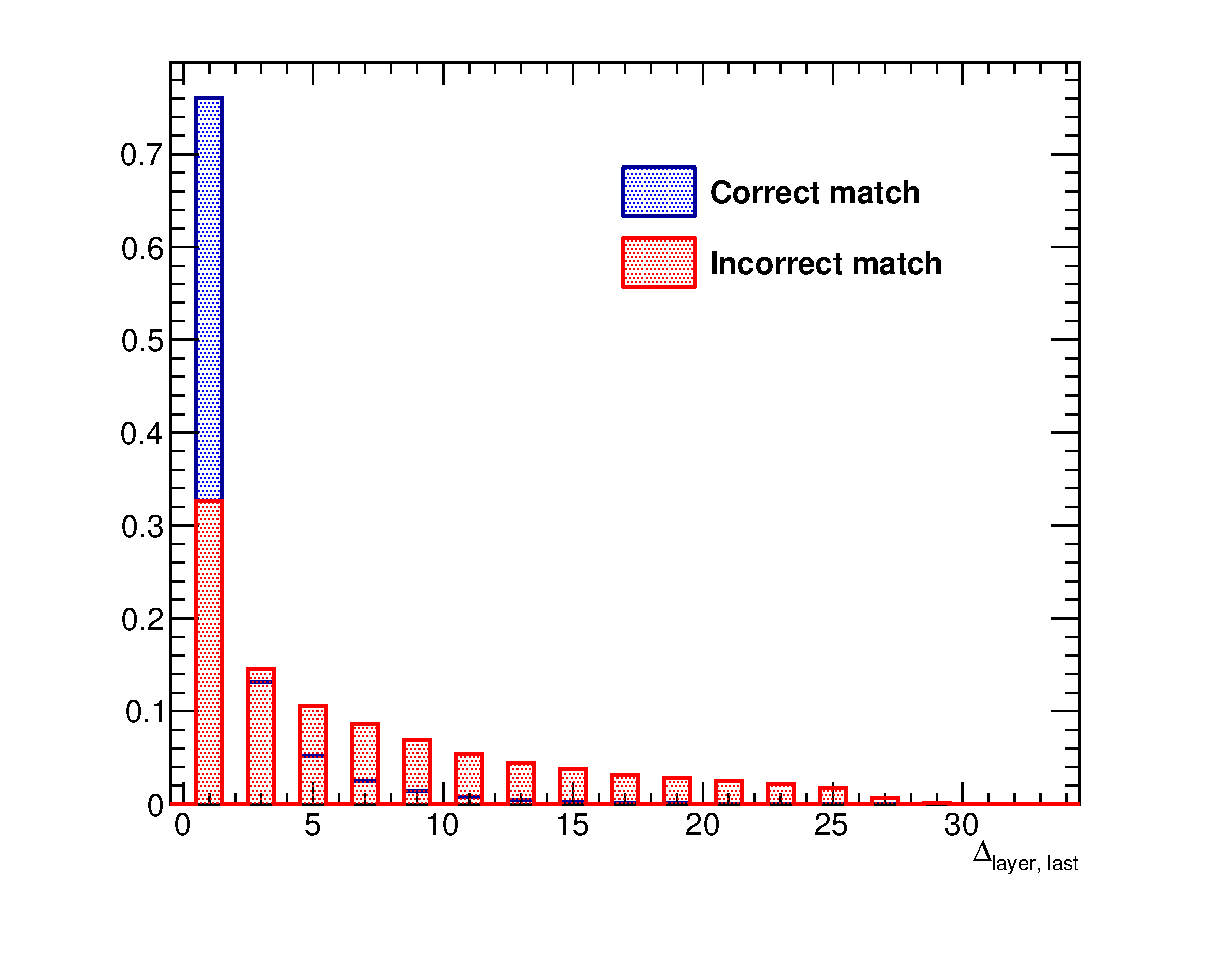
\includegraphics[width=7cm]{images/hough_3d_matching/3DMatching_Barrel_2Track_DLL_Separation.eps} \label{fig:3DMatchingBarrel2TrackDLLSeparation}}
  \hspace{1em}
  \subfloat[$\Delta_{\textrm{layer, last}}$ probability density distribution.  The peak of the distribution aligns well with the correct matches peak in Fig.~\ref{fig:3DMatchingBarrel2TrackDLLSeparation} which aides in maximising the number of correct matches made.]{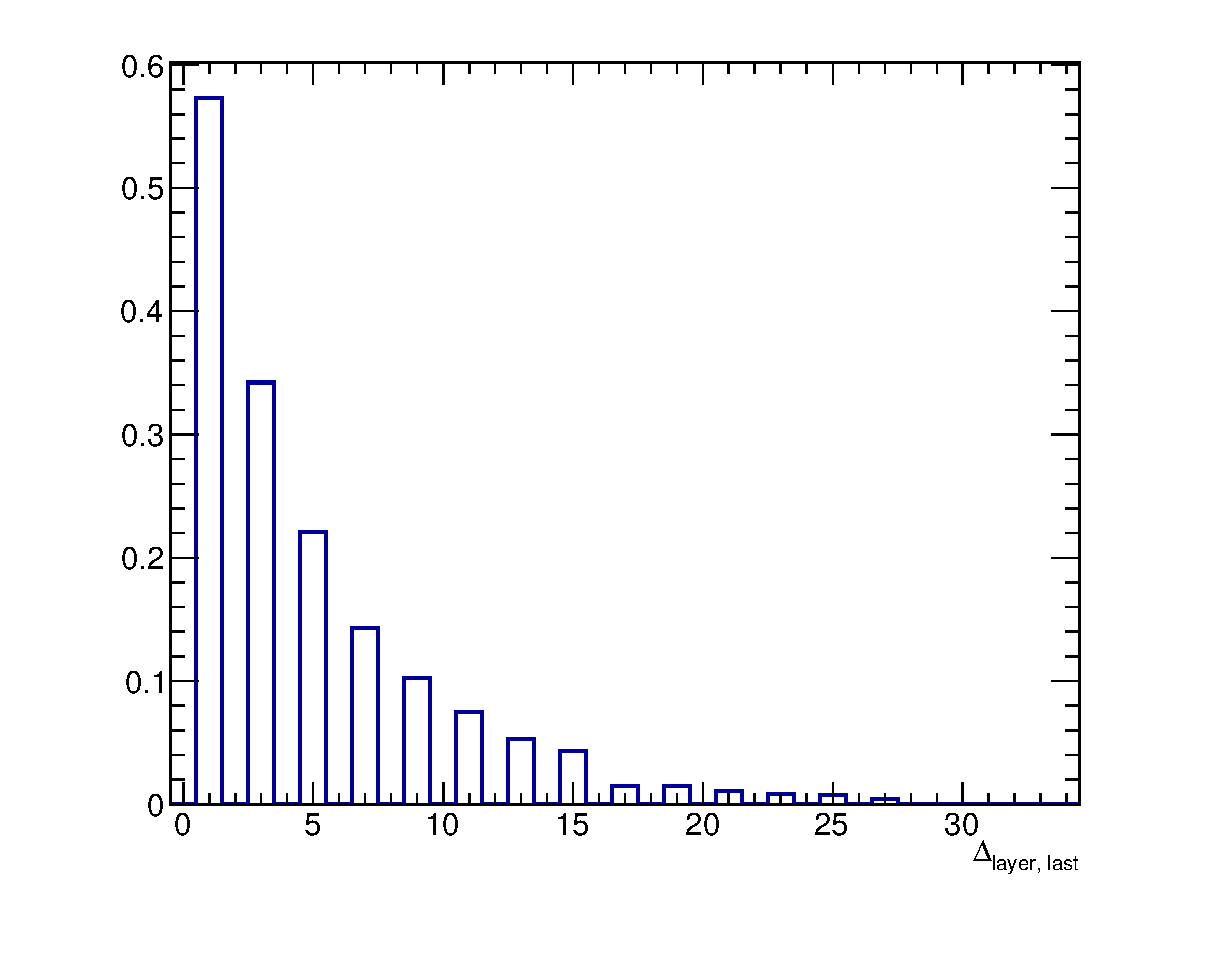
\includegraphics[width=7cm]{images/hough_3d_matching/3DMatching_Barrel_2Track_DLL_PDF.eps} \label{fig:3DMatchingBarrel2TrackDLLPDF}}
  \caption{$\Delta_{\textrm{layer, last}}$ and its probability density distribution in the barrel ECal for the two track case.  NEUT-based simulation of ND280 beam events were used to produce the distributions.}
  \label{fig:DLL}
\end{figure}
The third and final input to the likelihood, called $\Delta_{\textrm{layer, last}}$, is the difference in the ending layer of each 2D track which forms the matching candidate pair, where the ending layer refers to the layer furthest from the ND280 Tracker.  Functionally, how this function is used is essentially identical to $\Delta_{\textrm{layer, last}}$ so it will not be described in detail.  The separation ability of this variable and its corresponding probability density function for the two track, barrel case are shown in Fig.~\ref{fig:3DMatchingBarrel2TrackDLLSeparation} and Fig.~\ref{fig:3DMatchingBarrel2TrackDLLPDF} respectively.
\newline
\newline
The matching likelihood, $\mathcal{L}$, for a matching candidate pair is then
\begin{equation}
  \mathcal{L} = \mathcal{L}_{Q_{\textrm{ratio}}} \times \mathcal{L}_{\Delta_{\textrm{layer, first}}} \times \mathcal{L}_{\Delta_{\textrm{layer, last}}}.
\end{equation}
As described above, $\mathcal{L}$ is calculated for every matching candidate pair and the pair which maximise $\mathcal{L}$ is selected as a match and removed from the pool.  The process is then repeated until no more matches can be made.
\newline
\newline
3D tracks have now been formed, but the associated directions and positions of those tracks still need to be calculated.  The track fitting process for the newly formed 3D tracks is very similar to that described in section~\ref{subsec:ECal3DHitReconstruction}.  The tracks are briefly separated into their constituent 2D views and a charge-weighted average position of each layer is calculated using the track's constituent hits.  Then, the hits in the opposing view are used to estimate the third coordinate of a given layer using a least-squares fit.  After all of the coordinates have been estimated, a full 3D least-squares fit of the positions in each layer is performed to estimate the 3D track's direction and position in that ECal layer.

\subsection{Track splitting}
\label{subsec:TrackSplitting}
During development of the reconstruction, it became clear that a certain topology had been overlooked.  An example of this is shown in Fig.~\ref{fig:MergedTrackEventDisplay} which shows a MC neutrino interaction in the ECal with 3 charged final states.  As can be seen from Fig.~\ref{fig:MergedTrackEventDisplay}, the muon (solid green line) is emitted back-to-back with one of the final-state protons (solid blue line) in this ECal view.  Because the Hough transform implementation only concerns itself with straight lines, the result is that such back-to-back trajectories are typically reconstructed as a single track.  However, there are two views available for every ECal module and the back-to-back emittance typically only appears in the ECal view which is perpendicular to the beam direction (the XY view).  So, the correctly reconstructed tracks in the other ECal view can be used to split the tracks in the problematic view.  
\begin{figure}
  \centering
  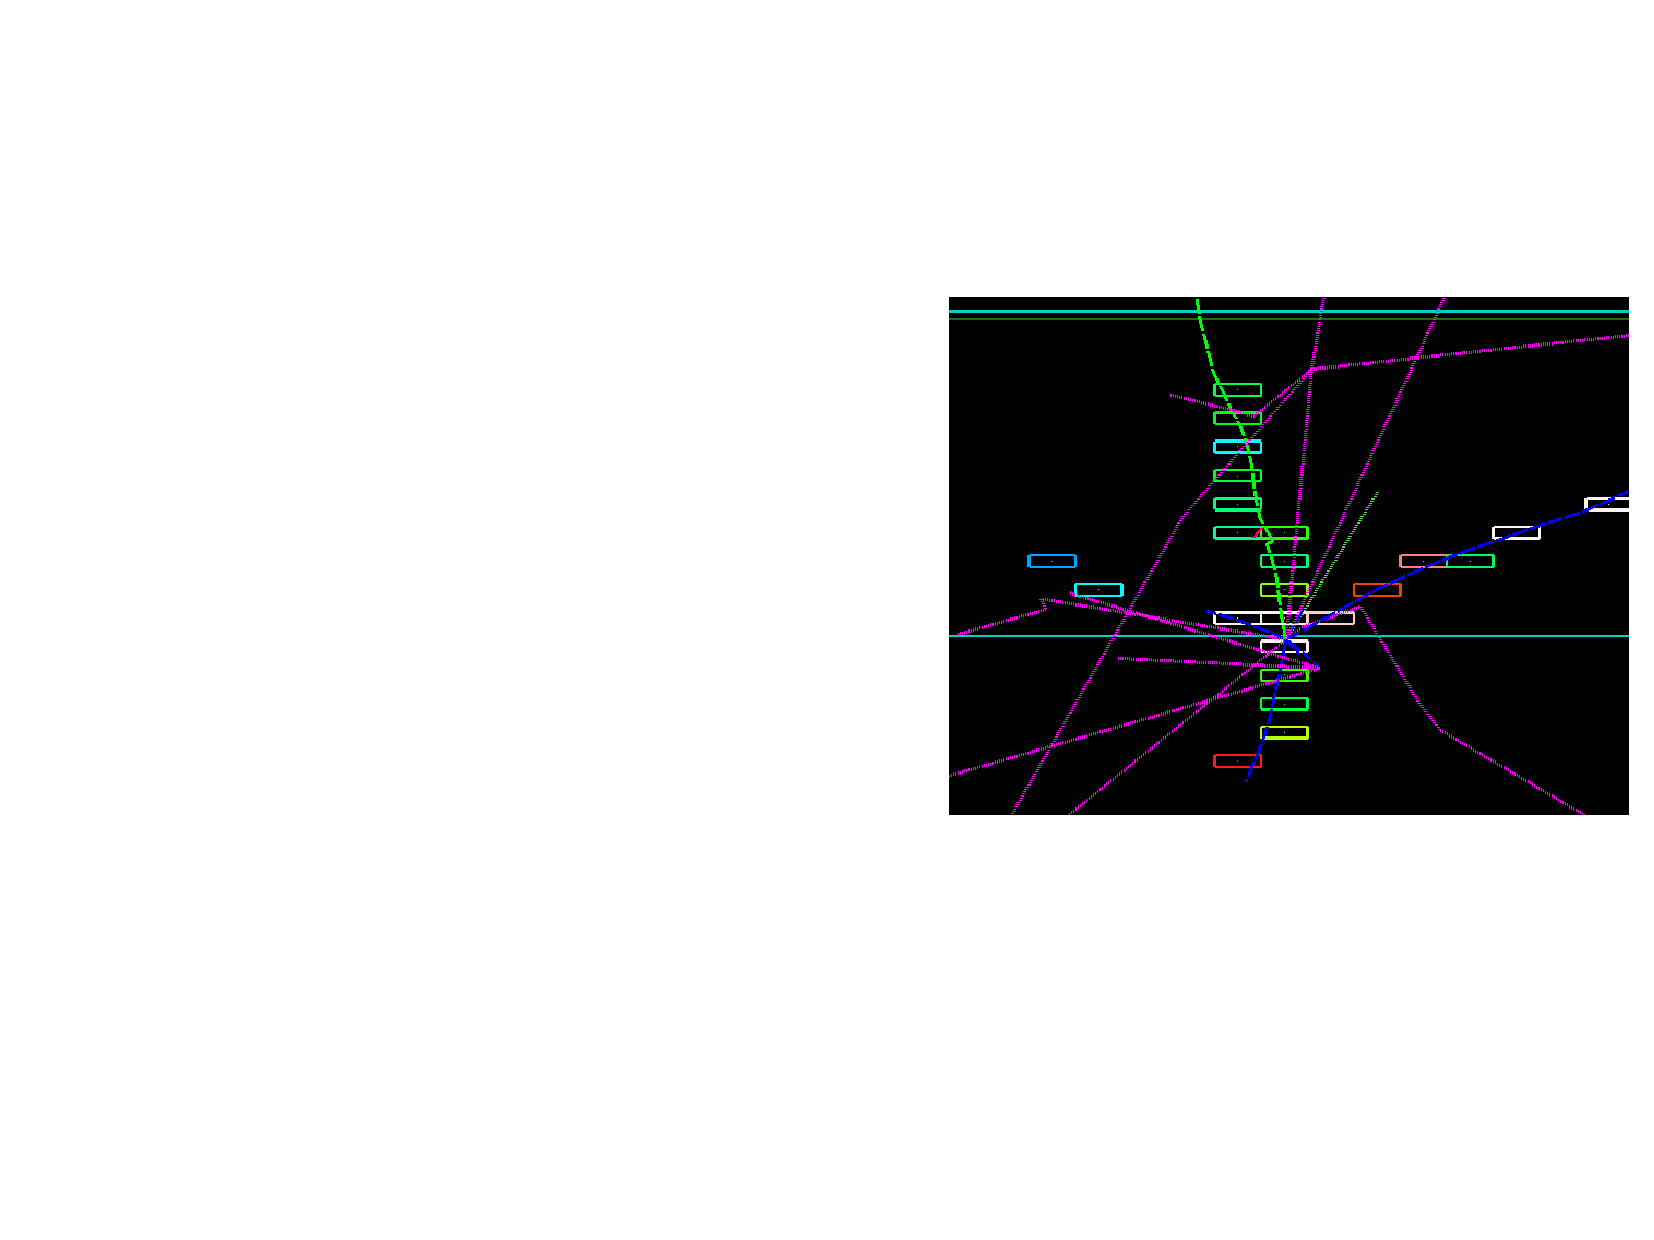
\includegraphics[width=10cm]{images/hough_3d_matching/MergedTrackEventDisplay.pdf}
  \caption{Event display (XY view) of a problematic (for the reconstruction) neutrino interaction in the ECal.  The solid green track is the muon, the solid blue tracks are protons and the pink tracks are neutrons.  The neutrino is the short dashed green line.  The proton travelling vertically downwards and the muon are created almost back to back leaving a line of hit scintillator bars.  The 2D hough transform would register this as a single straight line.}
  \label{fig:MergedTrackEventDisplay}
\end{figure}
\newline
\newline
Consider a neutrino interaction with two charged final-states which has been reconstructed as one track in one view (called the merged view) but reconstructed as two tracks in the other view (called the other view).  It should be expected that the single track in the merged view is not a particularly good match for either of the tracks in the other view.  However, if the two tracks in the other view were temporarily merged together and this new track was compared to the single track in the merged view, one should expect this match to return a much higher value of $\mathcal{L}$.  This feature can be used to identify a potentially merged track in a given view.
\newline
\newline
This motivated an extension to the 3D matching aspect of the reconstruction.  As a reminder, the 3D matching algorithm makes every pairwise comparison of tracks from each view to find the pair which maximise $\mathcal{L}$.  This matching routine was modified to also include temporary mergings of every pairwise combination of tracks in a single view.  These temporary mergings can then be compared to every single track in the other view.  As an example, consider a situation where 3 tracks (labelled $A$, $B$ and $C$) have been reconstructed in one view and two tracks (labelled $Y$ and $Z$) have been reconstructed in the other view.  With the old method, the following comparisons would be made:
\begin{equation}
\begin{split}
A &\longleftrightarrow Y \\
A &\longleftrightarrow Z \\
B &\longleftrightarrow Y \\
B &\longleftrightarrow Z \\
C &\longleftrightarrow Y \\
C &\longleftrightarrow Z
\end{split}
\label{eq:TrackSplittingOldMethod}
\end{equation}
With the new method, which includes temporarily merged pairs of tracks in a given view, the following comparisons would be made:
\begin{equation}
\begin{split}
A &\longleftrightarrow Y \\
A &\longleftrightarrow Z \\
B &\longleftrightarrow Y \\
B &\longleftrightarrow Z \\
C &\longleftrightarrow Y \\
C &\longleftrightarrow Z \\
A+B &\longleftrightarrow Y \\
A+B &\longleftrightarrow Z \\
A+C &\longleftrightarrow Y \\
A+C &\longleftrightarrow Z \\
B+C &\longleftrightarrow Y \\
B+C &\longleftrightarrow Z \\
A &\longleftrightarrow Y+Z \\
B &\longleftrightarrow Y+Z \\
C &\longleftrightarrow Y+Z
\end{split}
\label{eq:TrackSplittingNewMethod}
\end{equation}
In terms of the matching comparisons, the temporarily merged comparisons are treated on the same footing as the single track comparisons; $\mathcal{L}$ is calculated for each comparison and the one which maximises $\mathcal{L}$ is selected.  However, the post-matching treatment of the best match depends on whether a temporary merge is involved.  If the match which maximises $\mathcal{L}$ involves two single tracks then the treatment is as before; they are removed from the pool and the process is repeated.  If a temporarily merged pair are involved, the 2D crossing location of the temporarily merged tracks is calculated and is then used to split the single track in the other view.  The original track is removed from the pool and replaced by the two single tracks formed from the split.  The matching process is then begun again and repeated until all matches have been made.

\subsection{Track pairwise crossing reconstruction}
\label{subsec:TrackCrossingReconstruction}
The final step of the reconstruction is to estimate where each of the 3D track's paths cross.  As each track is reconstructed as a straight line in 3D, the final step is fairly simple.  Using the track direction and position information calculated at the end of section~\ref{subsec:3DHoughTrackReconstruction}, the position at closest approach for every pairwise combination of 3D tracks is calculated analytically.  The distance of closest approach is also calculated.  Six hits, the closest three from each 3D track, are then associated to the pairwise crossing. 

\section{Output of the reconstruction}
\label{sec:ReconOutput}
The reconstruction is run over every 3D cluster found in the ECal.  By applying the steps outlined above, for each 3D cluster the following output is given:
\begin{itemize}
  \item A set of 3D tracks
  \item The pairwise crossings of all 3D tracks found in the cluster
\end{itemize}
Note that no vertex formation beyond the pairwise crossings is calculated at this stage, nor is any analysis of the 3D tracks performed.  While this may seem like an oversight of the reconstruction, this approach was decided as no assumptions are made about what the tracks/crossings represent at this point, making the output more generic.  Any analysis which wants to make use of the reconstruction is given enough information to apply more targeted reconstruction downstream. 


%
%To build the probability density distributions, the output of the 2D reconstruction was used to form every possible matching pair (as described above) and the results were separated into two distinct categories: correctly matched and incorrectly matched.
\section{Validation of the reconstruction}
\label{sec:ReconstructionValidation}
Because of the large scope of the reconstruction and the limited time available for the presented analysis, the validation of the reconstruction was done in parallel to the rest of the analysis and is still an ongoing effort.  The validation that has been done can be split into two areas: validation of the performance of the algorithms purely using MC and comparisons of MC to data using control samples.
\subsection{Validation of algorithm performance}
\label{subsec:ValidationOfAlgorithmPerformance}
The first performance validation investigated the angular resolution using the enhanced reconstruction (by L. Pickering).  This study calculated the angular resolution for MC muons fired into the side-left ECal for a range of entry angles.  For each MC event, the cosine of the angular separation between the true particle angle and the reconstructed angle was calculated, $\cos\theta^{\textrm{Sep}}$.  The values of $\cos\theta^{\textrm{Sep}}$ were then binned in a distribution.  An outward scan from the peak of the distribution was then performed to find where the height decreased to $68\%$ of the peak.  The value of $\theta^{\textrm{Sep}}$ and this point was taken as the angular resolution.  These results are shown in Fig.~\ref{fig:MuonAngularResolutionDSECal}.  Generally speaking, the found angular resolutions are very good.  For long trajectories (200~mm), the angular resolution is within 15$^\circ$.  It is only for short tracks (40~mm) that the angular resolution becomes large.
\begin{figure}
  \centering
  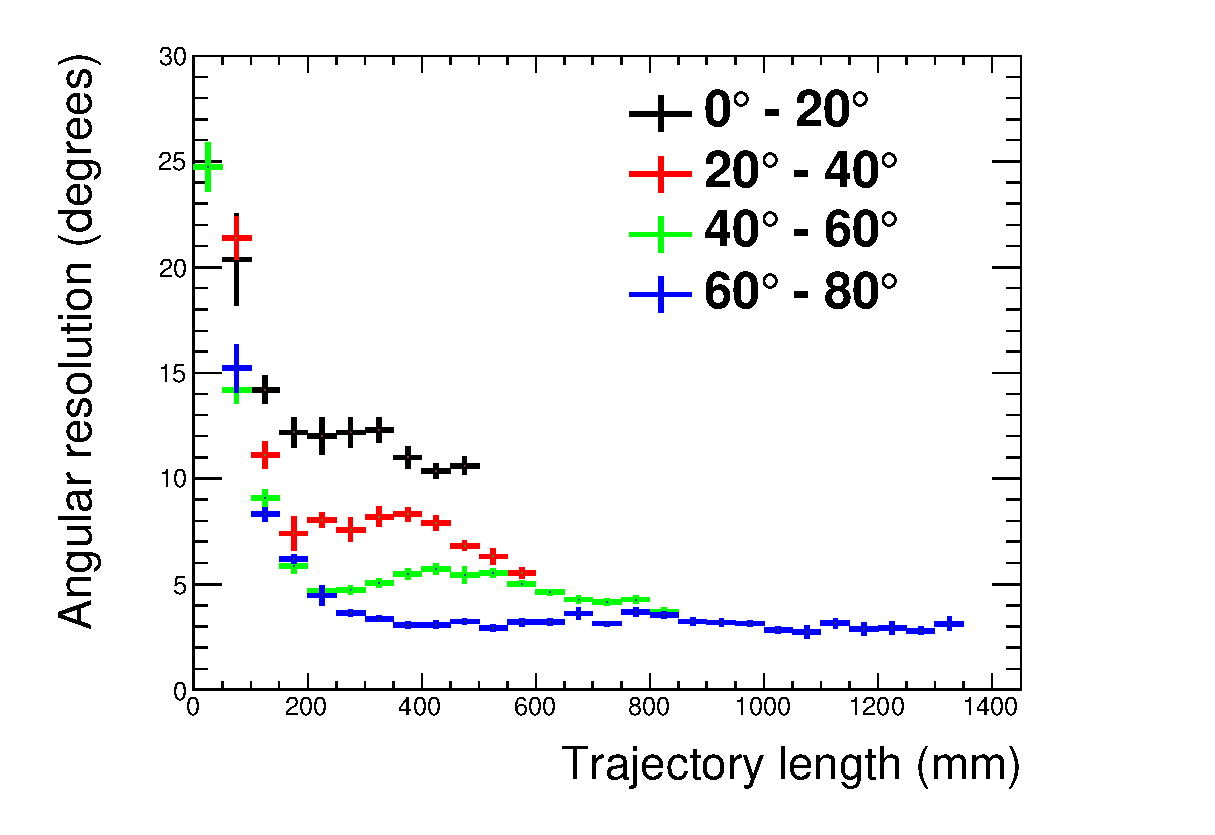
\includegraphics[width=12cm]{images/hough_validation/MuonAngularResolutionDSECal}
  \caption{The angular resolution as a function of trajectory length in the DS ECal when applying the enhanced reconstruction to muon MC.  The colour coding refers to the true entry angle range of the muons.  The figure was generated using single muon particle gun fired into the front face of the DS ECal with a controlled range of entry angles.  The angular resolution distributions were created by L. Pickering.}
  \label{fig:MuonAngularResolutionDSECal}
\end{figure}
\newline
\newline
The second performance validation studied the success of the 3D matching.  To do this, a sample of beam MC events in the ECals were processed through the enhanced reconstruction.  After completion, the 2D components of the 3D tracks were analysed and matched to the true particles which created them.  A match was counted as a success if both 2D components were matched to the same true particle.  These results are shown in table~\ref{table:PercentageCorrect3DMatching}, separated out by which track matching likelihood was used.  For the 1 and 2 track likelihood cases, the matching performs very well.  It is only in cases where the 3 track likelihood is used that the matching start to suffer slightly.  However, all of the correct matching rates are well above 50$\%$ which suggests that the 3D matching is performing adequately. 
\begin{table}
  \begin{tabular}{c | c c c }
   & 1 track likelihood & 2 track likelihood & 3 track likelihood \\ \hline \hline
   $1^{\textrm{st}}$ track matched& 96$\%$ & 92$\%$ & 80$\%$ \\
   $2^{\textrm{nd}}$ track matched&  & 89$\%$ & 79$\%$ \\
   $3^{\textrm{rd}}$ track matched&  &  & 70$\%$ \\
  \end{tabular}
  \caption{The percentage number of correct matches in the 3D matching separated by which track matching likelihood was used.  NEUT-based Monte Carlo simulation of the T2K beam was used to calculate the matching percentages.}
  \label{table:PercentageCorrect3DMatching}
\end{table}

\subsection{Data-motivated validation of the algorithms}
\label{subsec:DataMotivatedValidation}
As described above, the validation is still an ongoing effort and, so far, all of the data-motivated validation has been done by L. Pickering.  At time of writing, validation events  measured in ND280 can be split into two groups:
\begin{enumerate}
\item \textbf{FGD collinear cosmics (named fgdcol):} A sample of clean FGD-triggered cosmic events which are scaled to have an equal distribution of angles.
\item \textbf{Through-going Tracker muons (named bskmu):} A sample of clean beam-triggered events which solely contain a muon depositing energy in TPC2, TPC3 and the DS ECal.
\end{enumerate}
The fgdcol sample will naturally contain a good sample of barrel ECal events whilst having only a limited number of DS ECal events whereas the reverse is true for the bskmu sample.  So, it follows that the fgdcol and bskmu samples should be used to separately assess the reconstruction in the barrel ECal and DS ECal respectively. 
\newline
\newline
Fig.~\ref{fig:TotalChargeDataValidation} shows the summed charge contained in all tracks reconstructed in each ECal cluster.  To clarify what this means, if a reconstructed ECal cluster contained three reconstructed tracks where tracks 1, 2 and 3 contain 20~MEU, 50~MEU and 30~MEU of charge respectively, that event would be registered as having 100~MEU of charge in the relevant distribution in Fig.~\ref{fig:TotalChargeDataValidation}.  Both the barrel ECal and DS ECal samples show a large discrepancy around the charge peak.  This offset can be explained as a hit-level charge discrepancy between data and Monte Carlo and is not caused by the reconstruction.  This discrepancy should, however, be considered during analysis of the systematic uncertainties.  Unfortunately, the DS ECal events in the bskmu sample (Fig.~\ref{fig:TotalChargebskmuDS}) shows an extra data excess in the 20~MEU to 30~MEU region which is just before the charge peak.  This data excess can not be explained by a relative hit inefficiency. 
\begin{figure}%
  \centering
  \subfloat[Barrel ECal events in the fgdcol sample.  The data peak is offset \YoshiFinal{from }{ADDRESSED - was `to'} the Monte Carlo peak, indicating an unmodelled dead channel issue.]{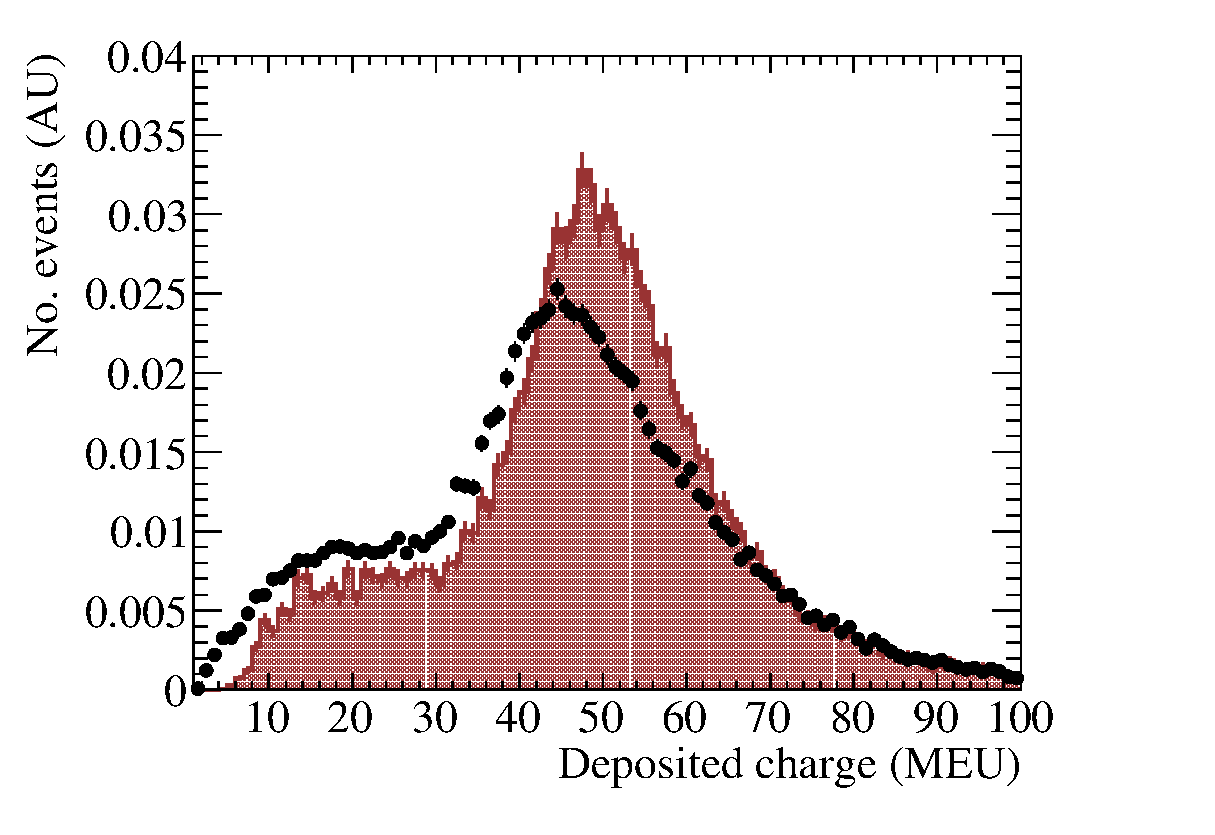
\includegraphics[width=7.5cm]{images/hough_validation/TotalCharge_fgdcol_Barrel.eps} \label{fig:TotalChargefgdcolBarrel}}
  \hspace{1em}
  \subfloat[DS ECal events in the bskmu sample.  The data peak is offset \YoshiFinal{from }{ADDRESSED - was `to'} the Monte Carlo peak, indicating an unmodelled dead channel issue.  There is also a significant data excess before the peak of the distributions.]{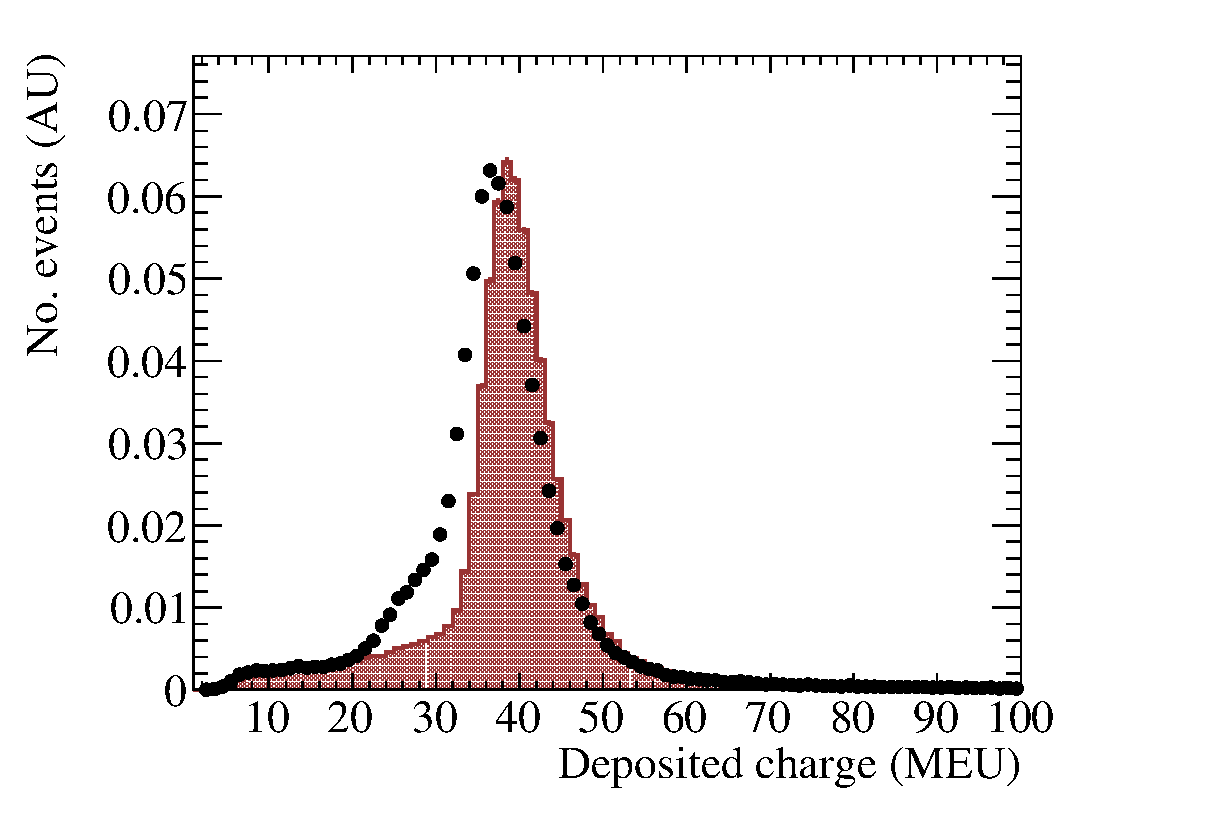
\includegraphics[width=7.5cm]{images/hough_validation/TotalCharge_bskmu_DSECal.eps} \label{fig:TotalChargebskmuDS}}
  \caption{The summed charge contained on all tracks reconstructed in each ECal cluster.  The red histograms and black points are Monte Carlo and data respectively.}
  \label{fig:TotalChargeDataValidation}
\end{figure}
\newline
\newline
Fig.~\ref{fig:TotalHitsDataValidation} shows the summed number of hits contained in all tracks reconstructed in each ECal cluster.  Generally speaking, the distributions in Fig.~\ref{fig:TotalHitsDataValidation} share similar features to those in Fig.~\ref{fig:TotalChargeDataValidation}.  Importantly, an excess of data events appears just before the peak in Fig.~\ref{fig:TotalHitsDataValidation}.  The fact that this excess also appears in Fig.~\ref{fig:TotalHitsDataValidation} strongly suggests that the issue is caused by the number of hits associated to the reconstructed tracks, rather than the deposited charge.  Further investigation of this discrepancy revealed that a mismodelled hit inefficiency, most likely due to dead DS ECal channels, was the issue.  One of the 2D track quality checks (see section~\ref{subsec:2DTrackQualityChecks}) requires that a 2D track candidate can not skip a layer in a given view which is problematic when considering dead channels.  
\begin{figure}%
  \centering
  \subfloat[Barrel ECal events in the fgdcol sample.  The only significant discrepancy is the offset of the data peak relative to the Monte Carlo peak, suggesting an unmodelled dead channel issue.]{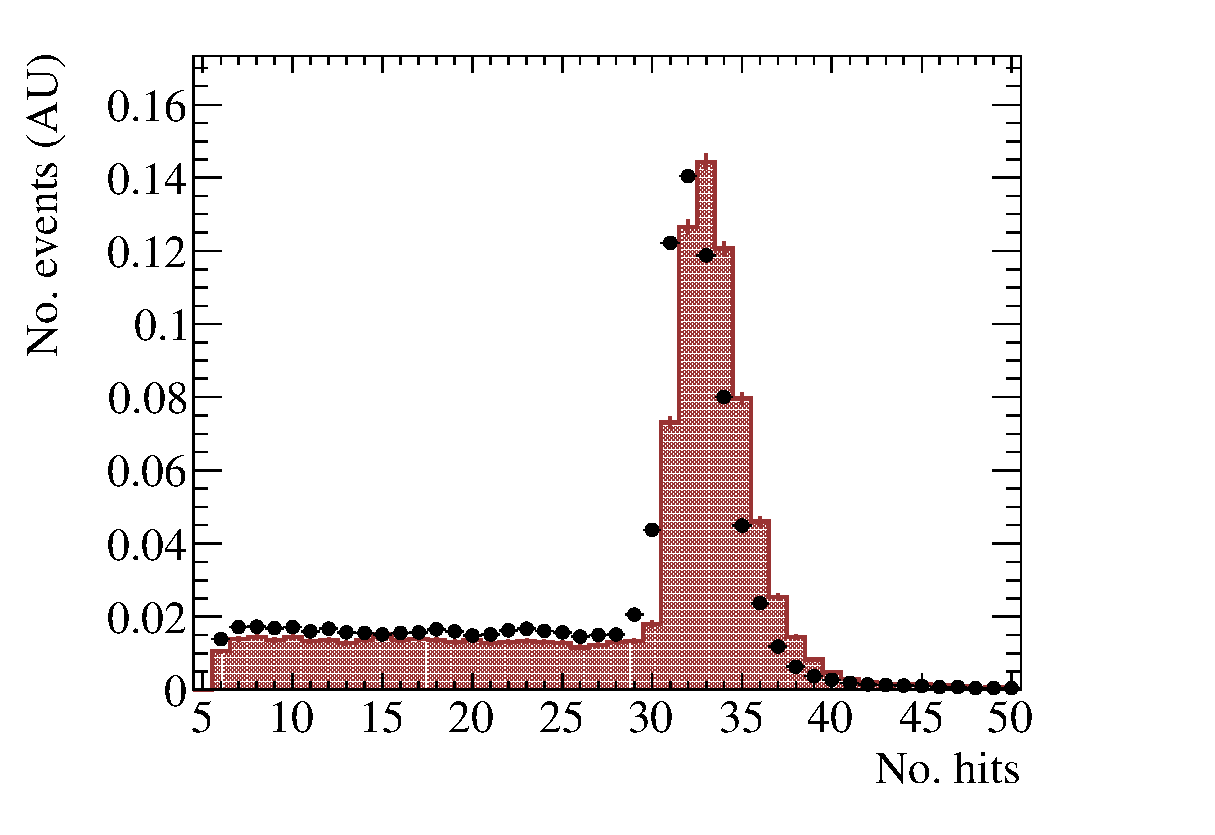
\includegraphics[width=7.5cm]{images/hough_validation/TotalHits_fgdcol_Barrel.eps} \label{fig:TotalHitsfgdcolBarrel}}
  \hspace{1em}
  \subfloat[DS ECal events in the bskmu sample.  There is a significant data excess before the peak in the distributions.]{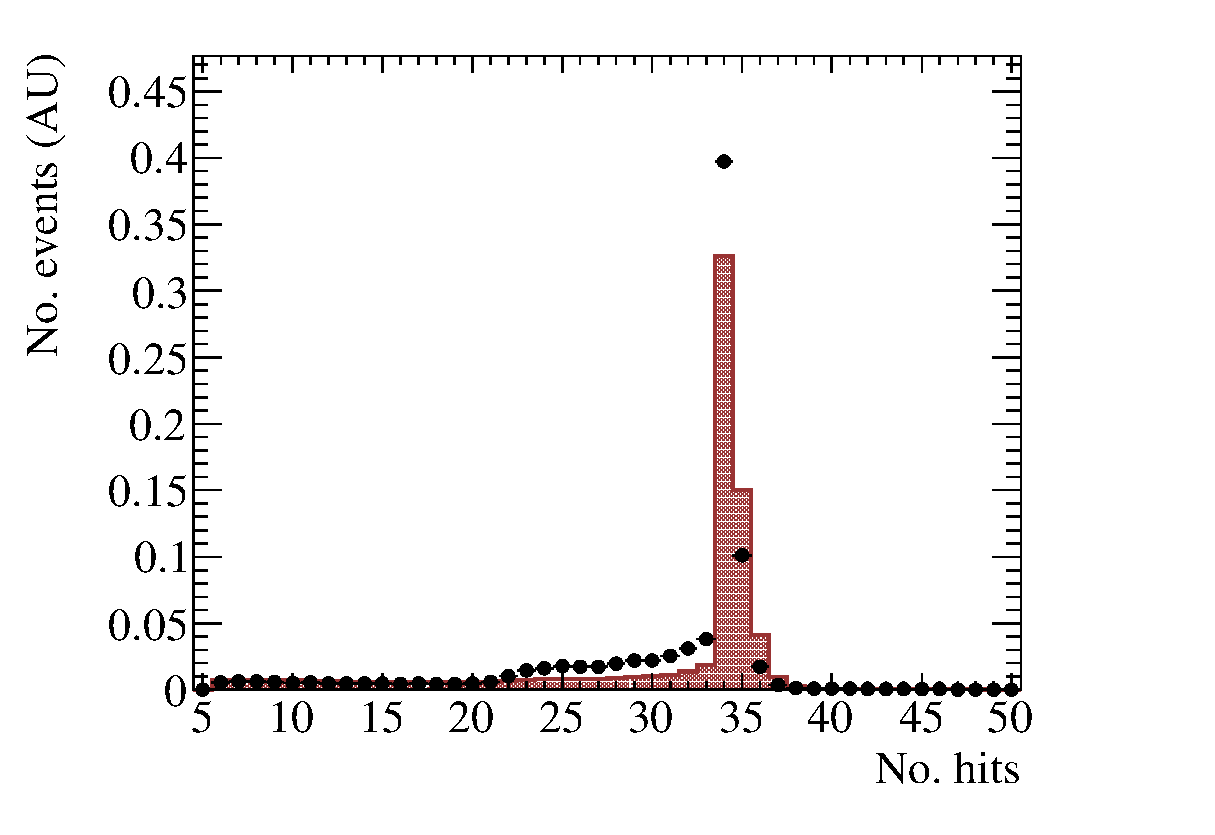
\includegraphics[width=7.5cm]{images/hough_validation/TotalHits_bskmu_DSECal.eps} \label{fig:TotalHitsbskmuDS}}
  \caption{The summed number of hits contained on all tracks reconstructed in each ECal cluster.  The red histograms and black points are Monte Carlo and data respectively.}
  \label{fig:TotalHitsDataValidation}
\end{figure}
\newline
\newline
To test this hypothesis, this requirement was relaxed to allow a 2D track candidate to skip a single ECal layer and the Monte Carlo bskmu sample was re-processed.  The re-processed DS ECal events are shown in Fig.~\ref{fig:bskmuCorrectedDSDataValidation}.  As can clearly be seen, the data excess before the peak in the distributions has now gone.  Unfortunately, large scale processing and analysis of beam Monte Carlo events had already started by the time this issue was discovered and so it was infeasible to include this bug fix in the analysis.  So, it was decided that this issue would be treated as an additional systematic uncertainty.  The collected data events were processed with this fix in place.
\begin{figure}[b!]%
  \centering
  \subfloat[Summed charge contained on all tracks in each reconstructed ECal cluster.]{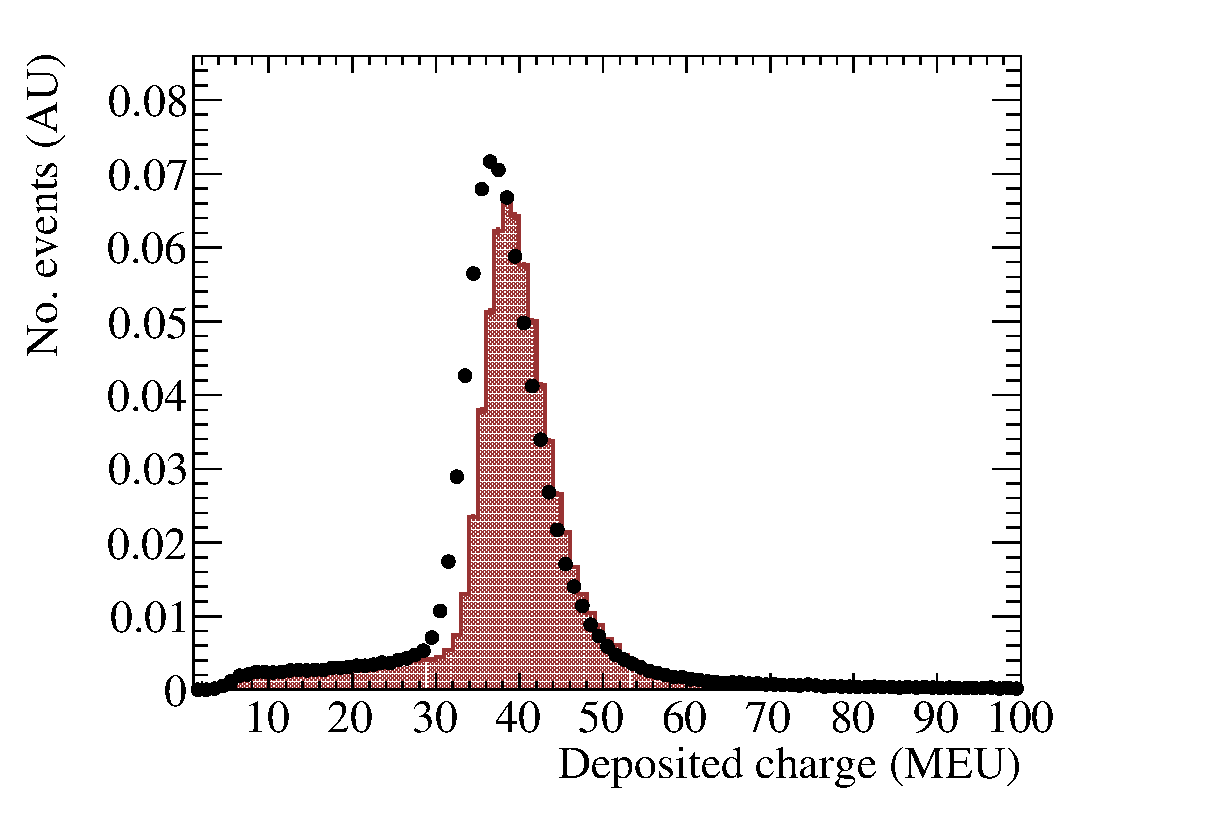
\includegraphics[width=7.5cm]{images/hough_validation/TotalCharge_bskmuCorrected_DSECal.eps} \label{fig:TotalChargebskmuCorrectedDS}}
  \hspace{1em}
  \subfloat[Summed number of hits contained on all tracks in each reconstructed ECal cluster.]{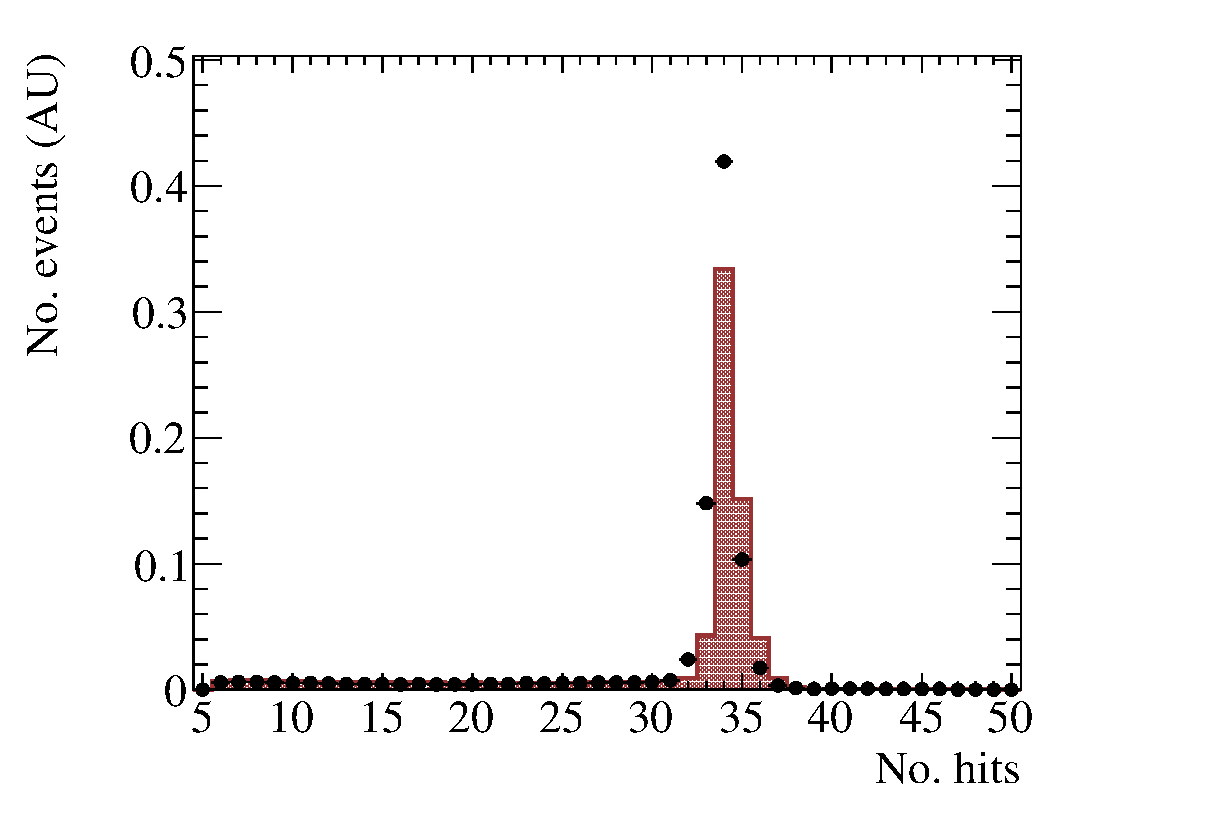
\includegraphics[width=7.5cm]{images/hough_validation/TotalHits_bskmuCorrected_DSECal.eps} \label{fig:TotalHitsbskmuCorrectedDS}}
  \caption{The number of DS ECal events in the bskmu sample after relaxing the 2D track quality check.  The red histograms and black points are the Monte Carlo and data respectively.  The track quality fix has corrected the data excesses in both distributions, leaving only the offset between the data and Monte Carlo peaks.}
  \label{fig:bskmuCorrectedDSDataValidation}
\end{figure}
